\documentclass[a4paper,oneside,12pt]{ThesisStyle}

\usepackage{amsmath,amssymb}             % AMS Math
\usepackage{bbm}
\usepackage[utf8]{inputenc}
\usepackage[T1]{fontenc}
\usepackage[ngerman]{babel}
\usepackage[left=1.0in,right=3.5cm,top=0.4in,bottom=1.1in,includefoot,includehead,headheight=13.6pt]{geometry}
\renewcommand{\baselinestretch}{1.05}

% Table of contents for each chapter

\usepackage[nottoc, notlof, notlot]{tocbibind}
\usepackage[german]{minitoc}
\setcounter{minitocdepth}{2}
\mtcindent=15pt
% Use \minitoc where to put a table of contents

\usepackage{aecompl}

% Glossary / list of abbreviations [Abk�rzungsverzeichnes]

\usepackage[intoc]{nomencl}
\let\abvz\nomenclature
\renewcommand{\nomname}{Abk{\"u}rzungsverzeichnes}
\setlength{\nomlabelwidth}{.25\hsize}
\renewcommand{\nomlabel}[1]{#1\dotfill}
\setlength{\nomitemsep}{-\parsep}

\makenomenclature

% include matlab code into Latex
\usepackage[framed]{mcode}
% My pdf code

\usepackage{ifpdf}

\ifpdf
  \usepackage[pdftex]{graphicx}
  \DeclareGraphicsExtensions{.png,.pdf,.jpg}
  \usepackage[a4paper,pagebackref,hyperindex=true]{hyperref}
\else
  \usepackage{graphicx}
  \DeclareGraphicsExtensions{.ps,.eps}
  \usepackage[a4paper,dvipdfm,pagebackref,hyperindex=true]{hyperref}
\fi

\graphicspath{{.}{images/}}

% Links in pdf
\usepackage{color}
\definecolor{linkcol}{rgb}{0,0,0.4} 
\definecolor{citecol}{rgb}{0.5,0,0} 

% Change this to change the informations included in the pdf file

% See hyperref documentation for information on those parameters

\hypersetup
{
bookmarksopen=true,
pdftitle="Realisation und Simulation einer Kaeltelast mit Kaeltespeicher im Energieversorgungsnetz",
pdfauthor="Juri STEBLAU",
pdfsubject="Creation of refrigerator simulation with MATLAB", %subject of the document
%pdftoolbar=false, % toolbar hidden
pdfmenubar=true, %menubar shown
pdfhighlight=/O, %effect of clicking on a link
colorlinks=true, %couleurs sur les liens hypertextes
pdfpagemode=None, %aucun mode de page
pdfpagelayout=SinglePage, %ouverture en simple page
pdffitwindow=true, %pages ouvertes entierement dans toute la fenetre
linkcolor=linkcol, %couleur des liens hypertextes internes
citecolor=citecol, %couleur des liens pour les citations
urlcolor=linkcol %couleur des liens pour les url
}

% definitions.
% -------------------

\setcounter{secnumdepth}{3}
\setcounter{tocdepth}{2}

% Some useful commands and shortcut for maths:  partial derivative and stuff

\newcommand{\pd}[2]{\frac{\partial #1}{\partial #2}}
\def\abs{\operatorname{abs}}
\def\argmax{\operatornamewithlimits{arg\,max}}
\def\argmin{\operatornamewithlimits{arg\,min}}
\def\diag{\operatorname{Diag}}
\newcommand{\eqRef}[1]{(\ref{#1})}
\usepackage{rotating}                    % Sideways of figures & tables
%\usepackage{bibunits}
%\usepackage[sectionbib]{chapterbib}          % Cross-reference package (Natural BiB)
%\usepackage{natbib}                  % Put References at the end of each chapter
                                         % Do not put 'sectionbib' option here.
                                         % Sectionbib option in 'natbib' will do.
\usepackage{fancyhdr}                    % Fancy Header and Footer

% \usepackage{txfonts}                     % Public Times New Roman text & math font
  
%%% Fancy Header %%%%%%%%%%%%%%%%%%%%%%%%%%%%%%%%%%%%%%%%%%%%%%%%%%%%%%%%%%%%%%%%%%
% Fancy Header Style Options

\pagestyle{fancy}                       % Sets fancy header and footer
\fancyfoot{}                            % Delete current footer settings

%\renewcommand{\chaptermark}[1]{         % Lower Case Chapter marker style
%  \markboth{\chaptername\ \thechapter.\ #1}}{}} %

%\renewcommand{\sectionmark}[1]{         % Lower case Section marker style
%  \markright{\thesection.\ #1}}         %

\fancyhead[LE,RO]{\bfseries\thepage}    % Page number (boldface) in left on even
% pages and right on odd pages
\fancyhead[RE]{\bfseries\nouppercase{\leftmark}}      % Chapter in the right on even pages
\fancyhead[LO]{\bfseries\nouppercase{\rightmark}}     % Section in the left on odd pages

\let\headruleORIG\headrule
\renewcommand{\headrule}{\color{black} \headruleORIG}
\renewcommand{\headrulewidth}{1.0pt}
\usepackage{colortbl}
\arrayrulecolor{black}

\fancypagestyle{plain}{
  \fancyhead{}
  \fancyfoot{}
  \renewcommand{\headrulewidth}{0pt}
}

\usepackage{algorithm}
\usepackage[noend]{algorithmic}

%%% Clear Header %%%%%%%%%%%%%%%%%%%%%%%%%%%%%%%%%%%%%%%%%%%%%%%%%%%%%%%%%%%%%%%%%%
% Clear Header Style on the Last Empty Odd pages
\makeatletter

\def\cleardoublepage{\clearpage\if@twoside \ifodd\c@page\else%
  \hbox{}%
  \thispagestyle{empty}%              % Empty header styles
  \newpage%
  \if@twocolumn\hbox{}\newpage\fi\fi\fi}

\makeatother
 
%%%%%%%%%%%%%%%%%%%%%%%%%%%%%%%%%%%%%%%%%%%%%%%%%%%%%%%%%%%%%%%%%%%%%%%%%%%%%%% 
% Prints your review date and 'Draft Version' (From Josullvn, CS, CMU)
\newcommand{\reviewtimetoday}[2]{\special{!userdict begin
    /bop-hook{gsave 20 710 translate 45 rotate 0.8 setgray
      /Times-Roman findfont 12 scalefont setfont 0 0   moveto (#1) show
      0 -12 moveto (#2) show grestore}def end}}
% You can turn on or off this option.
% \reviewtimetoday{\today}{Draft Version}
%%%%%%%%%%%%%%%%%%%%%%%%%%%%%%%%%%%%%%%%%%%%%%%%%%%%%%%%%%%%%%%%%%%%%%%%%%%%%%% 

%%%%%%%%%%%%%%%%%%%%%%%%%%%%%%%%%%%%%%%%%%%%%%%%%%%%%%%%%%%%%%%%%%%%%%%%%%%%%%%%%%%
% Matlab for shortc
\newcommand{\matlab}{\textsc{Matlab\textsuperscript{\textsf{\textregistered}}}\,}
\newcommand{\matref}[1]{\matlab-Code~\ref{#1}}
%\renewcommand{\todo}{\todo$\,$}
%%%%%%%%%%%%%%%%%%%%%%%%%%%%%%%%%%%%%%%%%%%%%%%%%%%%%%%%%%%%%%%%%%%%%%%%%%%%%%%%%%%


\newenvironment{maxime}[1]
{
\vspace*{0cm}
\hfill
\begin{minipage}{0.5\textwidth}%
%\rule[0.5ex]{\textwidth}{0.1mm}\\%
\hrulefill $\:$ {\bf #1}\\
%\vspace*{-0.25cm}
\it 
}%
{%

\hrulefill
\vspace*{0.5cm}%
\end{minipage}
}

\let\minitocORIG\minitoc
\renewcommand{\minitoc}{\minitocORIG \vspace{1.5em}}

\usepackage{multirow}
\usepackage{slashbox}

\newenvironment{bulletList}%
{ \begin{list}%
	{$\bullet$}%
	{\setlength{\labelwidth}{25pt}%
	 \setlength{\leftmargin}{30pt}%
	 \setlength{\itemsep}{\parsep}}}%
{ \end{list} }

\newtheorem{definition}{D�finition}
\renewcommand{\epsilon}{\varepsilon}

% centered page environment

\newenvironment{vcenterpage}
{\newpage\vspace*{\fill}\thispagestyle{empty}\renewcommand{\headrulewidth}{0pt}}
{\vspace*{\fill}}

% t_odo shit
\usepackage[textwidth=3.2cm]{todonotes}


%% i try \newfloat
%\floatstyle{plain}
%\usepackage{float}
%\newfloat{macode}{h}{mcd}[chapter]
%\floatname{macode}{Quellcode}
%
%% i try table of list of ..
%\usepackage{tocloft}
%\newcommand{\listmacode}{List of Quellcodes}
%\newlistof{mascode}{ex}{\listmacode}
%\newcommand{\mascode}[1]{%
%\refstepcounter{mascode}
%\par\noident\textbf{mascode \qqcode. #1}
%\addcontentsline{exp}{qcode}
%{\protect\number{\thechapter. \qqcode}#1}\par}


%%%%%%%%%%%%%%%%%%%%%%%%%%%%%%%%%%%%%%%%%%%%%%%%%%%%%%%%%%%%%%%%%%%%%%%%%%%%%%%%%%%%%%%%%%%%%%%%%%%%%%%%%%%%%%%%%%%%%%%%%%%%
% bebtex my try
\usepackage[nospace]{cite}
%%%%%%%%%%%%%%%%%%%%%%%%%%%%%%%%%%%%%%%%%%%%%%%%%%%%%%%%%%%%%%%%%%%%%%%%%%%%%%%%%%%%%%%%%%%%%%%%%%%%%%%%%%%%%%%%%%%%%%%%%%%%
\usepackage{multibib}
%%%%%%%%%%%%%%%%%%%%%%%%%%%%%%%%%%%%%%%%%%%%%%%%%%%%%%%%%%%%%%%%%%%%%%%%%%%%%%%%%%%%%%%%%%%%%%%%%%%%%%%%%%%%%%%%%%%%%%%%%%%%
% remember footnote and refer to that many times!
\newcommand{\footnoteremember}[2]{%
	\footnote{#2}%
	\newcounter{#1}%
	\setcounter{#1}{\value{footnote}}%
}
\newcommand{\footnoterecall}[1]{%
	\footnotemark[\value{#1}]%
}
%%%%%%%%%%%%%%%%%%%%%%%%%%%%%%%%%%%%%%%%%%%%%%%%%%%%%%%%%%%%%%%%%%%%%%%%%%%%%%%%%%%%%%%%%%%%%%%%%%%%%%%%%%%%%%%%%%%%%%%%%%%%%
\usepackage[ngerman]{cleveref}
%%%%%%%%%%%%%%%%%%%%%%%%%%%%%%%%%%%%%%%%%%%%%%%%%%%%%%%%%%%%%%%%%%%%%%%%%%%%%%%%%%%%%%%%%%%%%%%%%%%%%%%%%%%%%%%%%%%%%%%%%%%%%
\setcounter{secnumdepth}{5}
%%%%%%%%%%%%%%%%%%%%%%%%%%%%%%%%%%%%%%%%%%%%%%%%%%%%%%%%%%%%%%%%%%%%%%%%%%%%%%%%%%%%%%%%%%%%%%%%%%%%%%%%%%%%%%%%%%%%%%%%%%%%%
\newcommand{\pinstall}{\dot{Q}_0^)}%
%%%%%%%%%%%%%%%%%%%%%%%%%%%%%%%%%%%%%%%%%%%%%%%%%%%%%%%%%%%%%%%%%%%%%%%%%%%%%%%%%%%%%%%%%%%%%%%%%%%%%%%%%%%%%%%%%%%%%%%%%%%%%
\newcommand{\ptrans}{\dot{Q}_{Tr}}%
%%%%%%%%%%%%%%%%%%%%%%%%%%%%%%%%%%%%%%%%%%%%%%%%%%%%%%%%%%%%%%%%%%%%%%%%%%%%%%%%%%%%%%%%%%%%%%%%%%%%%%%%%%%%%%%%%%%%%%%%%%%%%
\newcommand{\pkalt}{\dot{Q}_{0}}%
%%%%%%%%%%%%%%%%%%%%%%%%%%%%%%%%%%%%%%%%%%%%%%%%%%%%%%%%%%%%%%%%%%%%%%%%%%%%%%%%%%%%%%%%%%%%%%%%%%%%%%%%%%%%%%%%%%%%%%%%%%%%%
\newcommand{\emehr}{Q_{mehr}}%
%%%%%%%%%%%%%%%%%%%%%%%%%%%%%%%%%%%%%%%%%%%%%%%%%%%%%%%%%%%%%%%%%%%%%%%%%%%%%%%%%%%%%%%%%%%%%%%%%%%%%%%%%%%%%%%%%%%%%%%%%%%%%
\newcommand{\pmehr}{\dot{Q}_{mehr}}%
%%%%%%%%%%%%%%%%%%%%%%%%%%%%%%%%%%%%%%%%%%%%%%%%%%%%%%%%%%%%%%%%%%%%%%%%%%%%%%%%%%%%%%%%%%%%%%%%%%%%%%%%%%%%%%%%%%%%%%%%%%%%%
\newcommand{\lmehr}{{W}_{mehr}}%
%%%%%%%%%%%%%%%%%%%%%%%%%%%%%%%%%%%%%%%%%%%%%%%%%%%%%%%%%%%%%%%%%%%%%%%%%%%%%%%%%%%%%%%%%%%%%%%%%%%%%%%%%%%%%%%%%%%%%%%%%%%%%
\newcommand{\lverd}{{W}_{Verd_{24}}}%
%%%%%%%%%%%%%%%%%%%%%%%%%%%%%%%%%%%%%%%%%%%%%%%%%%%%%%%%%%%%%%%%%%%%%%%%%%%%%%%%%%%%%%%%%%%%%%%%%%%%%%%%%%%%%%%%%%%%%%%%%%%%%
\newcommand{\lspez}{{W}_{spez_{24}}}%
%%%%%%%%%%%%%%%%%%%%%%%%%%%%%%%%%%%%%%%%%%%%%%%%%%%%%%%%%%%%%%%%%%%%%%%%%%%%%%%%%%%%%%%%%%%%%%%%%%%%%%%%%%%%%%%%%%%%%%%%%%%%%
\newcommand{\pnacht}{\dot{Q}_{Nacht}}%
%%%%%%%%%%%%%%%%%%%%%%%%%%%%%%%%%%%%%%%%%%%%%%%%%%%%%%%%%%%%%%%%%%%%%%%%%%%%%%%%%%%%%%%%%%%%%%%%%%%%%%%%%%%%%%%%%%%%%%%%%%%%%
\newcommand{\ptag}{\dot{Q}_{Tag}}%



%%%Uml sequence diagrams
%\usepackage{tikz}
%%\usetikzlibrary{arrows} % for pgf-umsld
%\usetikzlibrary{arrows,shadows} % for pgf-umsld
%\bususepackage[underline=true, rounded corners=false]{pgf-umlsd}


\begin{document}

\begin{titlepage}
	\begin{figure}[!ht]
		\parbox{0.5\textwidth}{
\includegraphics[height=2.4cm]{Title_Page/TU-logo_rot}}
		\qquad
		\begin{minipage}{0.4\textwidth}
			\begin{flushright}
				
\includegraphics[height=2.41cm]{Title_Page/sense}
			\end{flushright}
		\end{minipage}
	\end{figure}
	\begin{center}
		\vspace*{0.5cm}
		\noindent {\large \textbf{TECHNISCHE UNIVERSITÄT BERLIN}}\\
		\vspace*{0.3cm}
		\noindent {\large \textbf{Fachgebiet Energieversorgungsnetz und Integration Erneuerbarer Energien}}\\
		\vspace*{2.8cm}
		\noindent {\large  \textbf{STUDIENARBEIT}}\\
		\vspace*{1.0cm}
		\noindent {\huge \textbf{Objektorientierte Implementierung}}\\
		\vspace*{0.1cm}
		\noindent {\huge \textbf{und Simulation}}\\
		\vspace*{0.3cm}
		\noindent {\huge \textbf{einer Kältelast mit Kältespeicher}}\\
		\vspace*{0.05cm}
		\noindent {\Huge \textbf{im Energieversorgungsnetz}}\\
		\vspace*{1.8cm}
		\noindent \large vorgelegt von Juri \textsc{Steblau}\\
		\noindent \large Matr.-Nr: \textsc{300244}\\
		\vspace*{0.8cm}
		\noindent \large \today \\
		\vspace*{1.5cm}
	\end{center}
	\noindent \large \textbf{Korrektoren:} \\
	\begin{center}
		\noindent \large
		\begin{tabular}{llcl}
			\text{Advisor:} 	& Dipl.-Ing. 	Felix \textsc{Klein} 	& - & (TU-Berlin)\\
			\text{Examinator:} 	& Prof.Dr.-Ing. Kai \textsc{Strunz} 	& - & (TU-Berlin)\\
		\end{tabular}
	\end{center}
\setcounter{page}{0}
\end{titlepage}
\sloppy

\titlepage


\dominitoc

\pagenumbering{roman}

\cleardoublepage

\cleardoublepage
\begin{vcenterpage}
	\noindent\rule[2pt]{\textwidth}{0.5pt}
	\begin{center}
		{\large\textbf{Realisation und Simulation einer K\"altelast mit K\"altespeicher im Energieversorgungsnetz}}
	\end{center}
	\noindent\rule[2pt]{\textwidth}{0.5pt}
	{\large\textbf{Abstract:}}
	Hier bitte am Ende der Arbeit auf english die kurze Inhaltsangabe schreiben. \todo[caption={Abstract nicht da},
	color=green!30, inline]{ Hier muss noch ein Abstract rein !!!AM ENDE!!!}
	{\large\textbf{Keywords:}}
	Möglicherweise in Englisch! Fuck!\\
	\noindent\rule[2pt]{\textwidth}{0.5pt}
\end{vcenterpage}



\listoftodos
\tableofcontents
\listoffigures
\mtcaddchapter[Abbildungsverzeichnis] % damit wird eine Eintrag im Inhaltsverzeichniss erzeugt.
\listoftables
\mtcaddchapter[Tabellenverzeichnis]
\lstlistoflistings
\mtcaddchapter[\matlab-Code Verzeichnis]
\printnomenclature % to get this toc! makeindex hauptdokument.nlo -s nomencl.ist -o hauptdokument.nls
\mtcfixglossary[chapter] % solve the conflict of \minitoc and \nomencl

\mainmatter % maindocument whit arabic numbers

\chapter{Einleitung}
\label{chap:einleitung}

%%%%%%%%%%%%%%%%%%%%%%%%%%%%%%%%%%%%%%%%%%%%%%%%%%%%%%%
%%%%%%%%%%%%%%%%%%%%%%%%%%%%%%%%%%%%%%%%%%%%%%%%%%%%%%%
%%%%%%%%%%%%%%%%%%%%%%%%%%%%%%%%%%%%%%%%%%%%%%%%%%%%%%%
%\section*{Studiere DAS} \todo{dont forget to delete!}
Die Einleitung ist der wichtigste Textabschnitt einer Hochschularbeit – und zwar gleichgültig, ob es sich um eine Diplomarbeit,
eine Bachelorthesis oder eine Staatsexamensarbeit handelt. Hier wird der Leser ins Thema eingeführt, hier wird die Fragestellung
formuliert, und hier werden die methodischen Grundsatzentscheidungen getroffen.

Tipp: Man sollte die Einleitung, auch wenn das sogar von Prüferseite geäußert wird, nicht zum Schluss schreiben, sondern sie vorab
verfassen und sie während der Niederschrift als Arbeitsinstrument verwenden. Denn hieran – und nur hieran – zeigt sich, ob das
Untersuchungsvorhaben klappt. Häufig zeigt sich auch, weshalb es nicht so gut klappt.

All das weiß auch der Prüfer. Daher steht im Grunde die Note schon nach der Lektüre der Einleitung fest – zumindest wird es
schwierig sein, den Prüfer davon zu überzeugen, dass es sich doch um eine gute Arbeit handelt, wenn die Einleitung misslungen ist.
Aber wie schreibt man nun eine gute Einleitung? Im Folgenden einige grundlegende Hinweise:

Hilfreich ist eine Aufteilung in vier Teile, die sinnvoll aufeinander aufbauen. Das heißt nicht, dass es nicht auch andere
Möglichkeiten gibt, aber so funktioniert es mit Sicherheit – bei jedem Thema.  Das vorgeschlagene Schema sieht wie folgt aus:

\begin{enumerate}
	\item Hinführung (2 Absätze); diese besteht im Idealfall aus dem
		\begin{enumerate}
			\item Einstieg (etwas, was an die allgemeine Erfahrung anknüpft und unmittelbar ersichtlich ist) und
			\item einem weiteren Absatz, in dem – ausgehend vom Einstieg – auf das eigentliche Thema fokussiert wird.
		\end{enumerate}
		In einer Arbeit über Online-Marketing mit Facebook beispielsweise würde es im 1. Absatz um Online-Marketing allgemein gehen und im 2. Absatz
		auf die besonderen Anforderungen im Zusammenhang mit Facebook verwiesen. (Kontrollfrage: „Worum geht es hier?“)

	\item Fragestellung (1 Satz), auch als Problemstellung oder Forschungsfrage bezeichnet. Dabei handelt es sich im
		Idealfall tatsächlich nur um einen Satz oder einen Fragesatz. Die Fragestellung muss sich organisch aus dem 2. Absatz der Hinführung
		ableiten lassen. Im Idealfall ergibt sich für den Leser selbst angesichts des bisher Vermittelten an exakt dieser Stelle eine Frage, die er
		dann vom Verfasser bzw. der Verfasserin
		formuliert bekommt. Damit einher geht die Vorgabe, dass die Fragestellung wirklich nur exakt eine einzige Frage bzw. ein Forschungsproblem
		betrifft, nicht zwei oder drei. Wenn das passiert, hat man schon an dieser Stelle etwas falsch gemacht.  (Kontrollfrage: „Was ist das
		Problem?“)
	\item Operationalisierung der Fragestellung (3 bis 4 Sätze); dabei wird die Frage beantwortet, welche inhaltlichen und methodischen Aspekte im
		Zusammenhang mit der Klärung der Forschungsfrage wichtig sind. Dabei dürfen dann durchaus weiterführende Fragen gestellt oder Hypothesen
		formuliert werden, die sich aber wiederum
		auf die zentrale Fragestellung zurückführen lassen müssen. (Kontrollfragen: „Welche Überlegungen sind damit verknüpft? Was brauche ich, um
		die Forschungsfrage zu beantworten?“)
	\item Untersuchungsverlauf (pro Kapitel ein – kurzer – Absatz mit Verweis auf die Kapitelnummer); hier wird geklärt, was Inhalt der einzelnen
		Kapitel ist. Neue inhaltliche oder methodische Aspekte sollten hier nicht mehr vorkommen, hier geht es nur noch um das Wie, nicht mehr um
		das Was. (Kontrollfrage: „Wie wird
		vorgegangen?“)
\end{enumerate}

Hinweis: Die Schritte 3 und 4 werden häufig vermischt, oder die Operationalisierung unterbleibt ganz. Wir möchten nochmals deutlich
darauf hinweisen, dass die inhaltlichen, vor allem aber die methodischen und strukturellen Überlegungen in Bezug auf die
Fragestellung ein unverzichtbares Instrument sind, um die grundlegenden Zusammenhänge der Untersuchung zu klären. Demgegenüber
dient der Untersuchungsverlauf lediglich dazu, die Überlegungen im Hinblick auf die Gliederung in eine sinnvolle Abfolge zu
bringen.

Wie gesagt, dieses Schema funktioniert mit jedem Thema – wenn nicht, deutet das eher darauf hin, dass mit dem Thema etwas nicht
stimmt. Konkrete Fragen dazu beantworten wir gern im o:T-Forum. Ansonsten lässt sich auch im Rahmen einer Kurzberatung klären, ob
die Einleitung schlüssig ist. Dazu ist keine Beauftragung eines Lektorats notwendig.

% Don't forget to delete this!!!!

%%%%%%%%%%%%%%%%%%%%%%%%%%%%%%%%%%%%%%%%%%%%%%%%%%%%%%%
%%%%%%%%%%%%%%%%%%%%%%%%%%%%%%%%%%%%%%%%%%%%%%%%%%%%%%%
%%%%%%%%%%%%%%%%%%%%%%%%%%%%%%%%%%%%%%%%%%%%%%%%%%%%%%%
Die\todo{Einleitung mehrfach durchlesen!} Erforschung der Ursachen und der
Folgen des Klimawandels, die wachsende Schwierigkeit bei der Bereitstellung der
konventionellen Energien, die Neubewertung der Risiken und technischen Mitteln
bei der Endlagerung von Abfällen der Atomindustrie, die besorgniserregende
Erkenntnis der bisherigen Fehlbewertung der Atomsicherheit
\textcolor{red}{werden mit Gewissheit} die politisch beschlossene Förderung der
erneuerbaren Energien zu einer grundlegenden Energieform in den kommenden Jahren
in Deutschland und in Europa forcieren.\todo{Reicht so? Guck bitte nach oben.}

Der Umstieg auf alternative Energien ist mit einigen\todo{Bewertung
einfügen.}$\,$ Problemen verbunden. An einigen Orten ist der Einsatz dieser
Technik aus politischer, technischer, ökonomischer oder ökologischer Sicht nicht
möglich. Darum weichen oft die Stromerzeugung und der Strombedarf zeitlich und
räumlich voneinander ab. Windkraft im Meer, Wasserkraft in den Bergen,
Sonnenkraft in dem Süden, Geothermie in Island\todo{Der Satz ist scheiße,
umschreiben.}, Biomasse Land. Es ist auch eine Tatsache, dass nur ein Teil der
erneuerbaren Energien direkt vom Menschen beeinflusst werden kann. Besonders die
Menge der durch Sonne und Wind gewonnenen Energie schwankt abhängig von der
Wetterlage. Die Integration dieser Energie in Netz führt zur erhöhten
Bereitstellung an Regelenergie. Hauptsächlich wird diese Herausforderung durch
übermäßige Belastung der zur Ausregelung geeigneten konventionellen thermischen
Kraftwerke gelöst. Durch den regelungsbedingten ineffizienten Teillastbetrieb
und wiederholte An- und Abfahrvorgänge sinkt der Wirkungsgrad und ein höherer
Verschleiß der ist die Folge. Aus langfristiger Sicht wird
jedoch\todo[color=red!70,inline]{Das am Ende zur Ende schreiben} eine
Investition in Lastmanagement und in Energiespeicher unentbehrlich sein.

Brückentechnologien nicht sicher. Politischer Druck wächst. 


\chapter{Theorie}
\label{chap:theorie}
\minitoc

%%%%%%%%%%%%%%%%%%%%%%%%%%%%%%%%%%%%%%%%%%%%%%%%%%%%%%%%%%%%%%%%%%%%%%%%%%%%%%%%
%%%%%%%%%%%%%%%%%%%%%%%%%%%%%%%%%%%%%%%%%%%%%%%%%%%%%%%%%%%%%%%%%%%%%%%%%%%%%%%%

\section{Erneuerbare Energien im Energieversorgungsnetz}

Die Erneuerbaren Energien \"ubernehmen in Deutschland mit jedem Jahr einen
gr\"o\ss eren Anteil an der Elektrizit\"atsversorgung. Mehr als die H\"alfte der
Erneuerbaren Energie wird durch Wind und Photovoltaik erzeugt. Diese
Energiequellen sind jedoch im hohen Grad witterungsabh\"angig und k\"onnen stark
fluktuieren. Dadurch kann die Menge der zur Verf\"ugung stehenden Energie von
der Nachfrage zeitlich enorm abweichen. Der sichere Betrieb des Stromnetzes bei
einer konstanten Frequenz von $50\,Hz$ kann dadurch gef\"ardet werden.
Zus\"atzliche Bereitstellung an Regelleistung wird dadurch notwendig. Au\ss
erdem erfolgt die Erstellung der Fahrlpl\"ane f\"ur den Einsatz der
konventionellen Kraftwerke zwangsweise auf den fehlerbehafteten Vortagsprognosen
\"uber die Menge an Leistung aus Erneuerbaren Energien.  Die G\"ute der Prognose
bestimmt direkt den Regel- und den Reservebedarf.

%%%%%%%%%%%%%%%%%%%%%%%%%%%%%%%%%%%%%%%%%%%%%%%%%%%%%%%%%%%%%%%%%%%%%%%%%%%%%%%%
%%%%%%%%%%%%%%%%%%%%%%%%%%%%%%%%%%%%%%%%%%%%%%%%%%%%%%%%%%%%%%%%%%%%%%%%%%%%%%%%

\subsection*{Wetter- und Windprognose}

Eine exakte Prognose \"uber die Leistung aus Wind- und Photovoltaikanlagen setzt
eine nach M\"oglichkeit getreu Wettervorhersage voraus. In der Literatur wird
eine Genauigkeit f\"ur Day-Ahead Windleistungsprognose von $7\,\%$
\cite{prognose_doctor} und f\"ur Leistungsprognose aus Photovoltaikanlagen im
Bereich von $3.5\,\%\,-\,4.4\,\%$ \cite{solarvorhersagung} angegeben. Im
Verlaufe des Tages k\"onnen zeitweise deutlich h\"ohere Abweichungen auftreten.
Durch den gedrosselten Betrieb der Anlagen ist eine M\"oglichkeit zur
Kompensation der Prognosefehler gegeben. Der gedrosselte Anteil kann dadurch
jedoch nicht genutzt werden. Die Bereitstellung der Regelleistung durch
konventionelle oder andere Kraftwerke erscheint hier als sinnvoll. Eine bessere
L\"osung sind Energiespeicher, die bei \"Uberangebot Energie speichern und bei
einem Defizit Energie an das Netz freigeben.

Eine weitere M\"oglichkeit zur Reduzierung des obengenannten Effektes ist eine
variable Gestaltung der Netzlast. Kann sich ein Verbraucher nicht zu seinem
Nachteil dem Angebot der Energieerzeugung folgen, so würden die
Regelungsverluste und der Aufwand verringert und damit Kosten gespart werden.
Kann ein Verbraucher seine Hauptlast zeitlich verschieben, besteht das Potential
diese F\"ahigkeit zur Regelung einzusetzen.

Es ist vorstellbar, dass Anlagen zur K\"alteerzeugung auf Grund der thermischen
Tr\"agheit zu g\"unstigen Zeiten die Temperatur zus\"atzlich senken k\"onnen und
zu ung\"unstigen Zeiten die K\"uhlt\"atigkeit auf das Minimum herunterfahren.
Hiermit ist also das Interesse begr\"undet, das Lastverlagerungspotential in der
K\"alteerzeugung zu untersuchen.

%%%%%%%%%%%%%%%%%%%%%%%%%%%%%%%%%%%%%%%%%%%%%%%%%%%%%%%%%%%%%%%%%%%%%%%%%%%%%%%%
%%%%%%%%%%%%%%%%%%%%%%%%%%%%%%%%%%%%%%%%%%%%%%%%%%%%%%%%%%%%%%%%%%%%%%%%%%%%%%%%

\section{K\"alteerzeugung im Supermarkt: Potentiale und Besonderheiten}

Im Mittel entfallen $60\, \%$\cite{leghart, EANRW} des Stromverbrauchs in einem
Supermarkt auf Kühlen und Tiefkühlen von Produkten. Der durchschnittliche
Verbrauch in einem Supermarkt liegt zwischen 300 $MWh$ und 500 $MWh$ im
Jahr\cite{leghart}. In den kommenden Jahren sch\"atzt man den Wachstum des
gesamten K\"altebedarfs f\"ur Deutschland mit 100 \% \cite{probst}. Der Anteil
am Bedarf an elektrischen Energie vom Gesamtverbrauch eines Industrielandes für
Kälteerzeugung in den Supermärkten wird in der Literatur f\"ur  Australien mit
$1\, \%$ \cite{australia} und in Schweden mit $2\, \%$ \cite{doctor, EANRW}
Prozent angegeben. In Deutschland liegt der Verbrauch mit 6294 $GWh$ f\"ur das
Jahr 1999 bei rund $1.27\, \%$\cite{steilme}. Die Gr\"o\ss enordnung des
Verbrauchs f\"ur die Produktlagerung in Superm\"arkten und die M\"oglichkeit
diesen zeitlich zu verschieben, macht die Superm\"arkte f\"ur die Regelung
besonders interessant\todo{Eine \"Uberleitung finden}.

%%%%%%%%%%%%%%%%%%%%%%%%%%%%%%%%%%%%%%%%%%%%%%%%%%%%%%%%%%%%%%%%%%%%%%%%%%%%%%%%
%%%%%%%%%%%%%%%%%%%%%%%%%%%%%%%%%%%%%%%%%%%%%%%%%%%%%%%%%%%%%%%%%%%%%%%%%%%%%%%%

\subsection*{Beschr\"ankungen und Randbedingungen}

Die Mindesthaltbarkeit f\"ur bestimmten Produkte kann nur durch Lagerung
dieser Produkte in f\"ur sie festgelegtem K\"uhltemeperaturbereichen
garantiert werden. Dieser Temperaturbereich ist je nach Bedarf und Anwendung in
Normalk\"uhlung (NK\abvz{NK}{Normalk\"uhlung}) über 0 $\grad C$ und in
Tiefk\"uhlung (TK\abvz{TK}{Tiefk\"uhlung}) unter 0 $\grad C$ unterteilt. Auf der
nationalen und auch auf internationalen Ebene existieren Auflagen die die
maximale Temperaturen bei der Lagerung von Nahrungsmitteln vorschreiben. Die
fundamentale Verordnung ist die EG 853/2004. Aus der geht hervor, dass
normalgekühlte Produkte im Temperaturbereich 0 bis $+8$ $\grad C$ je nach
Nahrungsmittel und tiefgekühlte Produkte mindestens bei $-18$ $\grad C$ gekühlt
werden müssen.

Die K\"alteerzeugung im Supermarkt kann r\"aumlich generell in zwei Bereiche
unterteilt werden, dem Verkaufsbereich und dem Warenlager. Au\ss erdem kommen
K\"uhleinheiten zum Einsatz, die einer Verbundk\"alteanlage angeh\"oren oder
steckerfertig zur Verf\"ugung stehen. \"Uberwiegend werden im Verkaufsbereich
K\"uhlregale, K\"uhltruhen und K\"uhlschr\"anke im Tiefk\"uhlbereich und im
Niederk\"uhlbereich ebenso wie K\"uhltheken im Niederk\"uhlbereich installiert.
Zur Ausstattung z\"ahlen Ger\"ate in offener sowie durch T\"uren verschlie\ss
barer Ausf\"uhrung. Gro\ss enteils werden die die offenen Modelle au\ss erhalb
der \"Offnungszeiten durch Decken und Rollos zwecks Energieeinsparung
verschlossen.

%%%%%%%%%%%%%%%%%%%%%%%%%%%%%%%%%%%%%%%%%%%%%%%%%%%%%%%%%%%%%%%%%%%%%%%%%%%%%%%%
%%%%%%%%%%%%%%%%%%%%%%%%%%%%%%%%%%%%%%%%%%%%%%%%%%%%%%%%%%%%%%%%%%%%%%%%%%%%%%%%

\section{Objektorientierte Programmierung mit \matlab}

Seit Ende des letzten Jahrhunderts herrscht in der Fachliteratur für Informatik
die Meinung, dass der Einsatz von objektorientierten Techniken Programme
hervorbringt, die im Vergleich \textit{einfacher erweiterbar, besser testbar}
und \textit{besser wartbar} sind\todo{SIND, das ist hier nicht gut.}. Dabei wird
ein Verfahren angewendet, nach dem große Systeme in kleinere Teile des Ganzen
zerlegt werden. Programme lassen sich dadurch im Allgemeinen mit weniger Aufwand
und kleineren Fehlerwahrscheinlichkeit programmieren. Inspiriert durch die
Vorgänge aus der realen Welt, werden die Abläufe durch operierende Objekte
vorgestellt, die Aufträge erledigen und vergeben können. Die wesentlichen
Eigenschaften der objektorientierten Programmierung, kurz
OOP\abvz{OOP}{objektorientierte Programmierung}, sind die Datenkapselung, die
Polymorphie und die Vererbung.\footnote{ Ausführliche Informationen dazu findet
man z.B.  in \cite{OOP},\cite{java} oder \cite{python}.}

%%%%%%%%%%%%%%%%%%%%%%%%%%%%%%%%%%%%%%%%%%%%%%%%%%%%%%%%%%%%%%%%%%%%%%%%%%%%%%%%
%%%%%%%%%%%%%%%%%%%%%%%%%%%%%%%%%%%%%%%%%%%%%%%%%%%%%%%%%%%%%%%%%%%%%%%%%%%%%%%%

\subsection*{Allgemeine Erl\"auterungen}
\begin{description}

	\item[Klasse] Eine Klasse ist ein Instrument der
	Programmierung zur Erfassung von charakteristischen Eigenschaften
	zusammenh\"angender Objekte. Die Definition der Strukturen der Objekte
	erfolgt durch Klassen.

	\item[Objekt] Ein Objekt ist ein konkretes Exemplar einer
	Klasse.

	\item[Eigenschaften] Eigenschaften sind Variablen, die f\"ur jedes
	Objekt existieren, die von einer Klasse erzeugt werden.

	\item[Methoden] Methoden sind objektlokale Funktionen.

	\item[Datenkapselung] Der Zugriff auf Attribute einer Klasse erfolgt
	gew\"ohnlich durch ihre Methoden, die Kommunikationsschnittstellen
	darstellen. Dieses Verfahren bezeichnet man Datenkapselung.

	\item[Polymorphie] Wenn einem Objekt einer bestimmten Klasse die
	Objektvariablen einer anderen Klasse zugewiesen werden k\"onnen, spricht
	man von Polymorphie.

	\item[Vererbung] Die Vererbung erm\"oglicht durch Ver\"nderung der
	bestehenden Klassen neue Klassen zu erstellen. Die grundlegenden
	Programmteile der bestehenden Klasse werden zwangsl\"aufig
	\"ubernomen.\footnote{ Ausf\"urliche Informationen dazu findet man z.B.
	in \cite{pepperOOP}.}

\end{description}

%%%%%%%%%%%%%%%%%%%%%%%%%%%%%%%%%%%%%%%%%%%%%%%%%%%%%%%%%%%%%%%%%%%%%%%%%%%%%%%%
%%%%%%%%%%%%%%%%%%%%%%%%%%%%%%%%%%%%%%%%%%%%%%%%%%%%%%%%%%%%%%%%%%%%%%%%%%%%%%%%

\subsection*{Erl\"auterungen zur OOP-Syntax\footnote{ Es werden nur
Schl\"usselw\"orter vorgestellt, die essentiell sind. Eine tiefgreifende
Darstellung w\"urde den Rahmen einer Studienarbeit bei Weitem \"ubersteigen.
Ausf\"uhrliche Informationen dazu findet man z.B. in \cite{matlab_kompakt} oder
\url{http://www.mathworks.com/help/}.}}

\begin{description}

	\item[classdef] Neue Klassen werden mit der Anweisung
	\lstinline$classdef$ eingeleitet. Der Name der Klasse wird unmittelbar
	nach der Anweisung eingetragen. Der Klassen-Block endet mit der
	Anweisung \lstinline$end$.
	\item[properties] Die Anweisung \lstinline$properties$ beginnt den
	Eigenschaften-Block. Abgeschlossen wird der Block mit \lstinline$end$.
	Innerhalb einer Klasse k\"onnen mehrere Bl\"ocke existieren. M\"ochte
	man das Verhalten eines Eigenschaften-Blocks zus\"atzlich ver\"andern,
	ist der Einsatz von Attributen zweckm\"a\ss ig.
	\begin{lstlisting}[frame=none]
	properties (attribut1, attribut2, etc.)
	end
	\end{lstlisting}
	\item[methods] Die Anweisung \lstinline$methods$ beginnt den
	Methoden-Block und mit \lstinline$end$ wird er geschlossen. Analog zu
	dem Eigenschaften k\"onnen in einer Klasse mehrere Methoden-Bl\"ocke
	existieren. M\"ochte man das Verhalten eines Methoden-Blocks
	zus\"atzlich ver\"andern, ist der Einsatz von Attributen zweckm\"a\ss
	ig.
	\begin{lstlisting}[frame=none]
	methods (attribut1, attribut2, etc.)
	end
	\end{lstlisting}


\end{description}

%%%%%%%%%%%%%%%%%%%%%%%%%%%%%%%%%%%%%%%%%%%%%%%%%%%%%%%%%%%%%%%%%%%%%%%%%%%%%%%%
%%%%%%%%%%%%%%%%%%%%%%%%%%%%%%%%%%%%%%%%%%%%%%%%%%%%%%%%%%%%%%%%%%%%%%%%%%%%%%%%

\subsection*{Klassendefinition mit \matlab}

Klassen werden in \matlab mit Hilfe einer Datei mit der Endung $.m$ definiert,
die den selben Namen wie die Klasse hat. Im Quelltextbeispiel
\matref{Klassendefinition} wird eine Beispielklasse
\textbf{class\_name} mit einem Eigenschaften-Block und einem Methoden-Block
definiert.

\begin{lstlisting}[float=h!,caption={Beispiel Klassendefinition},label={Klassendefinition}, frame=none]
	classdef (Attributes) class_name < super_class % class definition
		properties (Attributes) % first property block
			PropertyName
		end % end of properties block
		% additionally here can be another methods block with 
		% specifying by another Attributes
		methods (Attributes) 
			function obj = class_name(obj,a) % consturctor
				obj.PropertyName = a;
			end
			function [X] = second_function(obj)
				X = obj.PropertyName + 1;
			end
		end
		% additionally here can be another methods block with 
		% specifying by another Attributes
	end % end of classdef block
\end{lstlisting}

%%%%%%%%%%%%%%%%%%%%%%%%%%%%%%%%%%%%%%%%%%%%%%%%%%%%%%%%%%%%%%%%%%%%%%%%%%%%%%%%
%%%%%%%%%%%%%%%%%%%%%%%%%%%%%%%%%%%%%%%%%%%%%%%%%%%%%%%%%%%%%%%%%%%%%%%%%%%%%%%%

\section{Anwendung der OOP am Modell}

In der \cref{vkb} wird ein einfaches Energieversorgungsnetz mit vier Knoten
dargestellt. Am Knoten eins ist eine regenerative elektrische Energiequelle, in
diesem Fall ein Windpark, angeschlossen. Weitere konventionelle elektrische
Energiequellen befinden sich an den Knoten zwei und drei. Die passiven Lasten
befinden sich am Knoten zwei und vier. Der Kältespeicher ist am Knoten zwei
angeschlossen. Im Bild wird der Kältespeicher Supermarkt durch einen
Einkaufswagen symbolisiert. Die Knoten sind untereinander durch Leitungen
verbunden.

\begin{figure}[h]
\caption{Vier Knoten Beispiel}
	\label{vkb}
	\begin{center}
	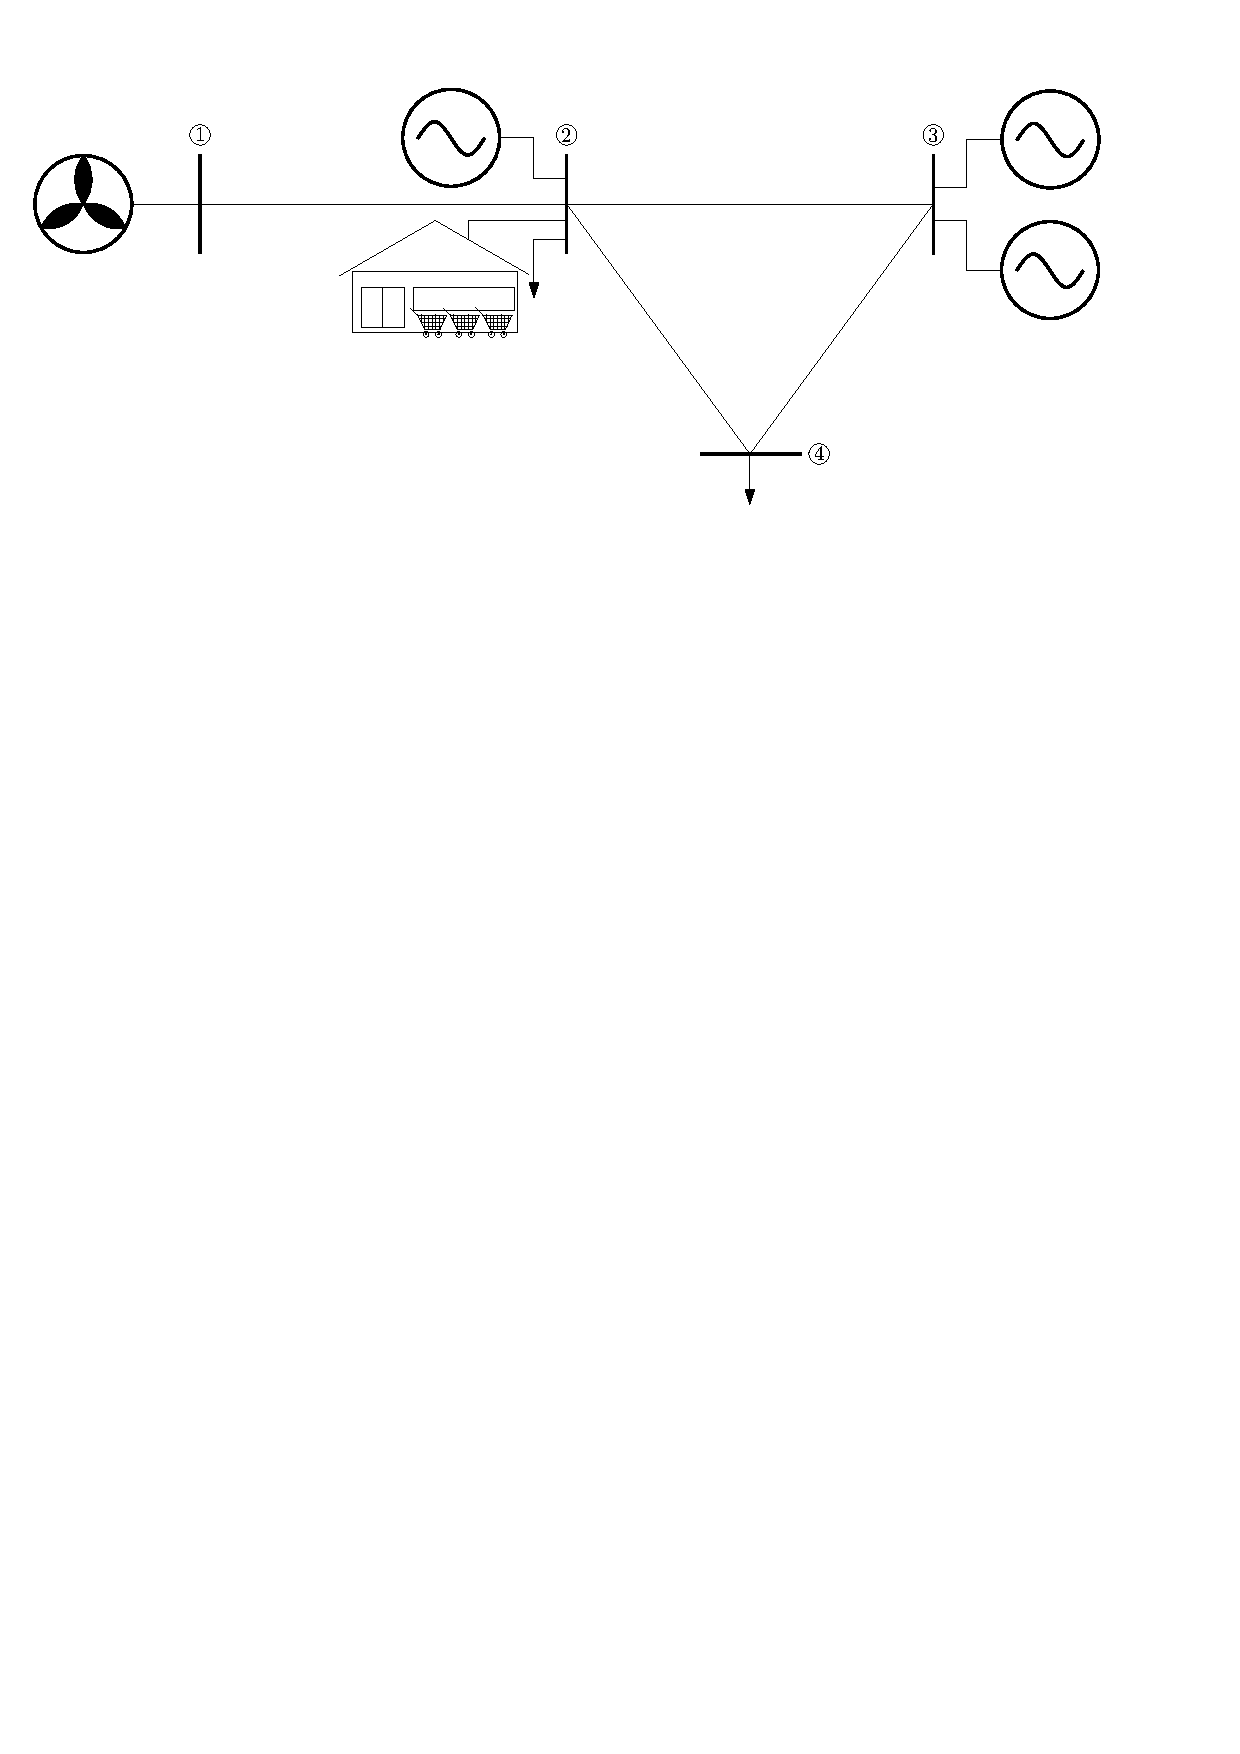
\includegraphics[scale=0.75]{images/SEVN/power_grid}
	\end{center}
\end{figure}

In der Realität kann ein Energieversorgungsnetz durch die Variation der
Knotenzahl und die Vermaschung beliebig komplizierte Form aufweisen. Bei der
Umsetzung der gegebenen Situation im Programm.

\begin{figure}[h]
\caption{Klassendiagramm Modellkonstrukt}
	\label{klassendiagramm}
	\begin{center}
	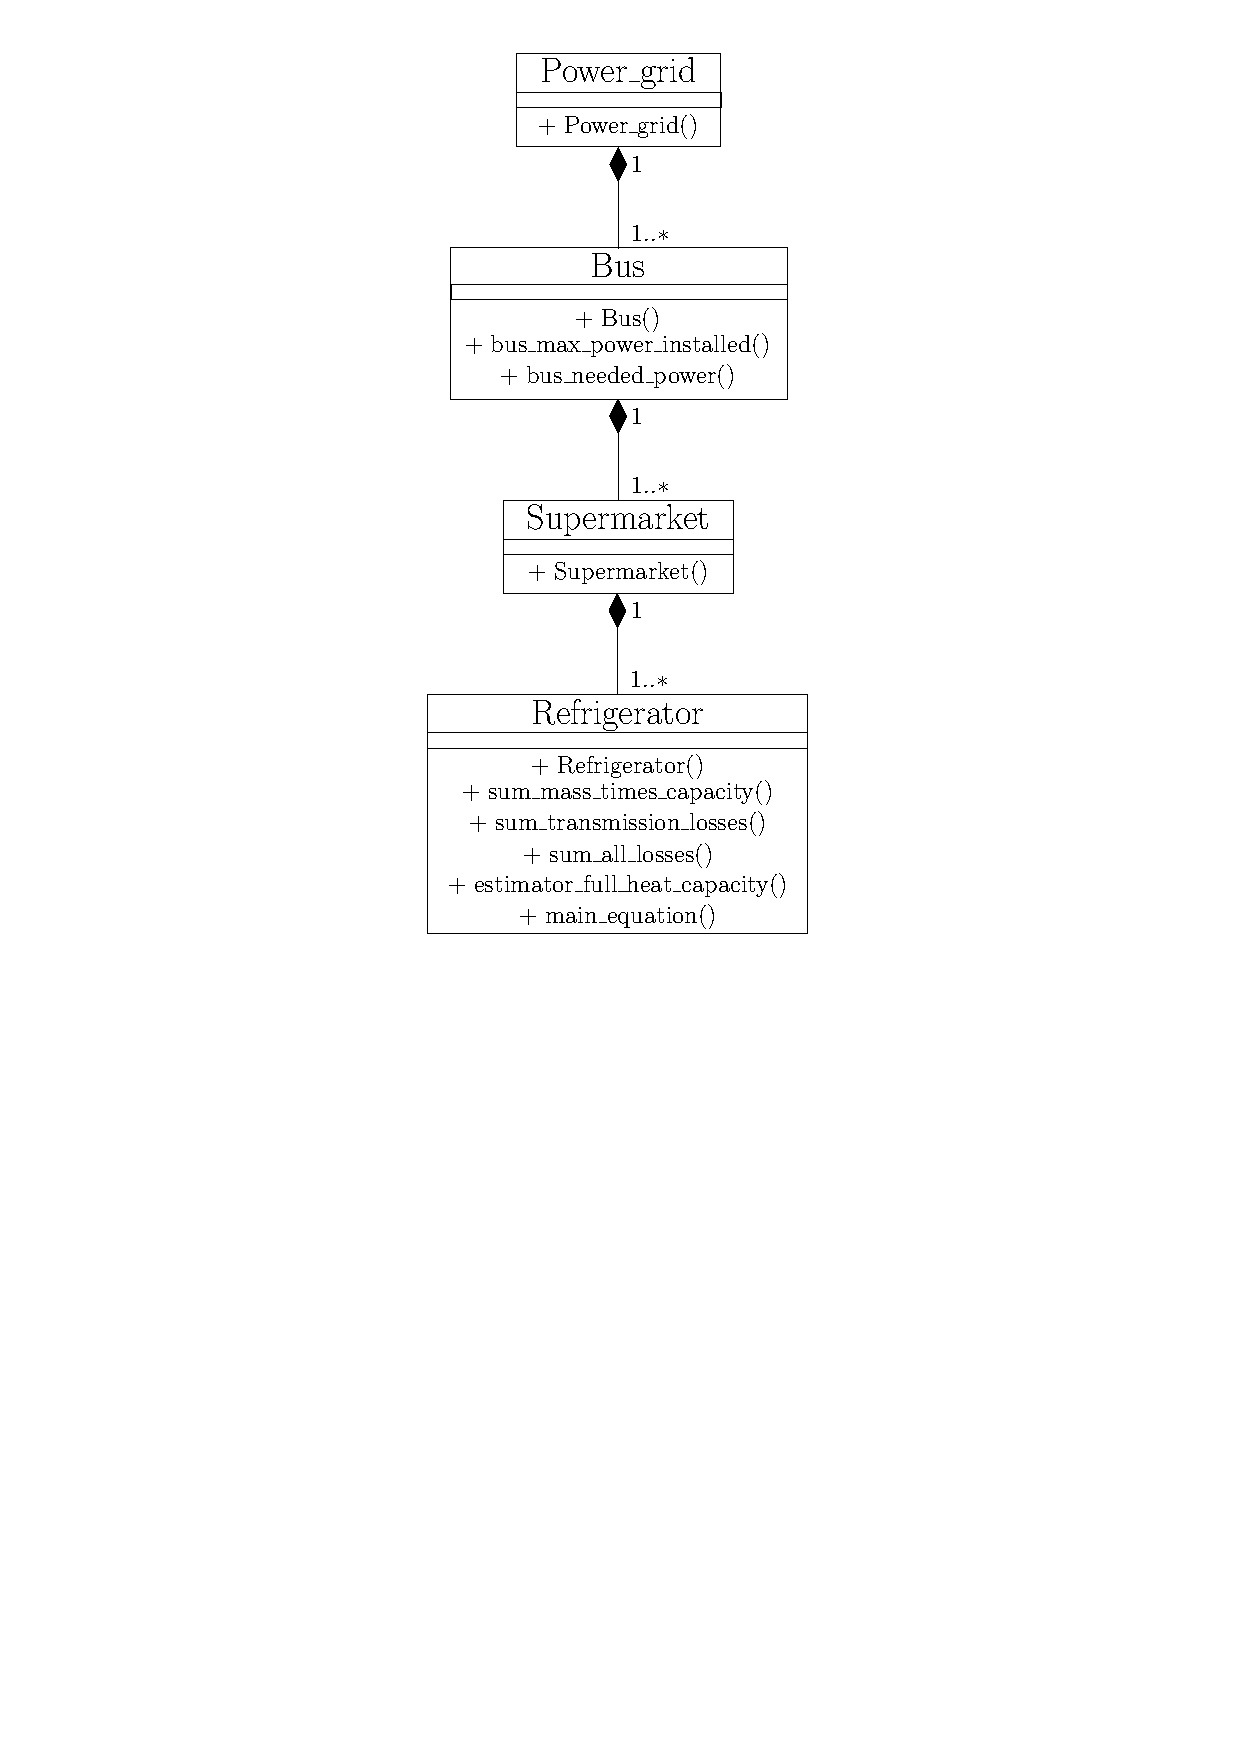
\includegraphics[scale=0.8]{images/Theorie_Super/class_diagramm}
	\end{center}
\end{figure}

Hier noch ein Zwischentext.

\begin{figure}[h]
\caption{Sequenzdiagramm Modellkonstrukt}
	\label{uml_sequence}
	\begin{center}
	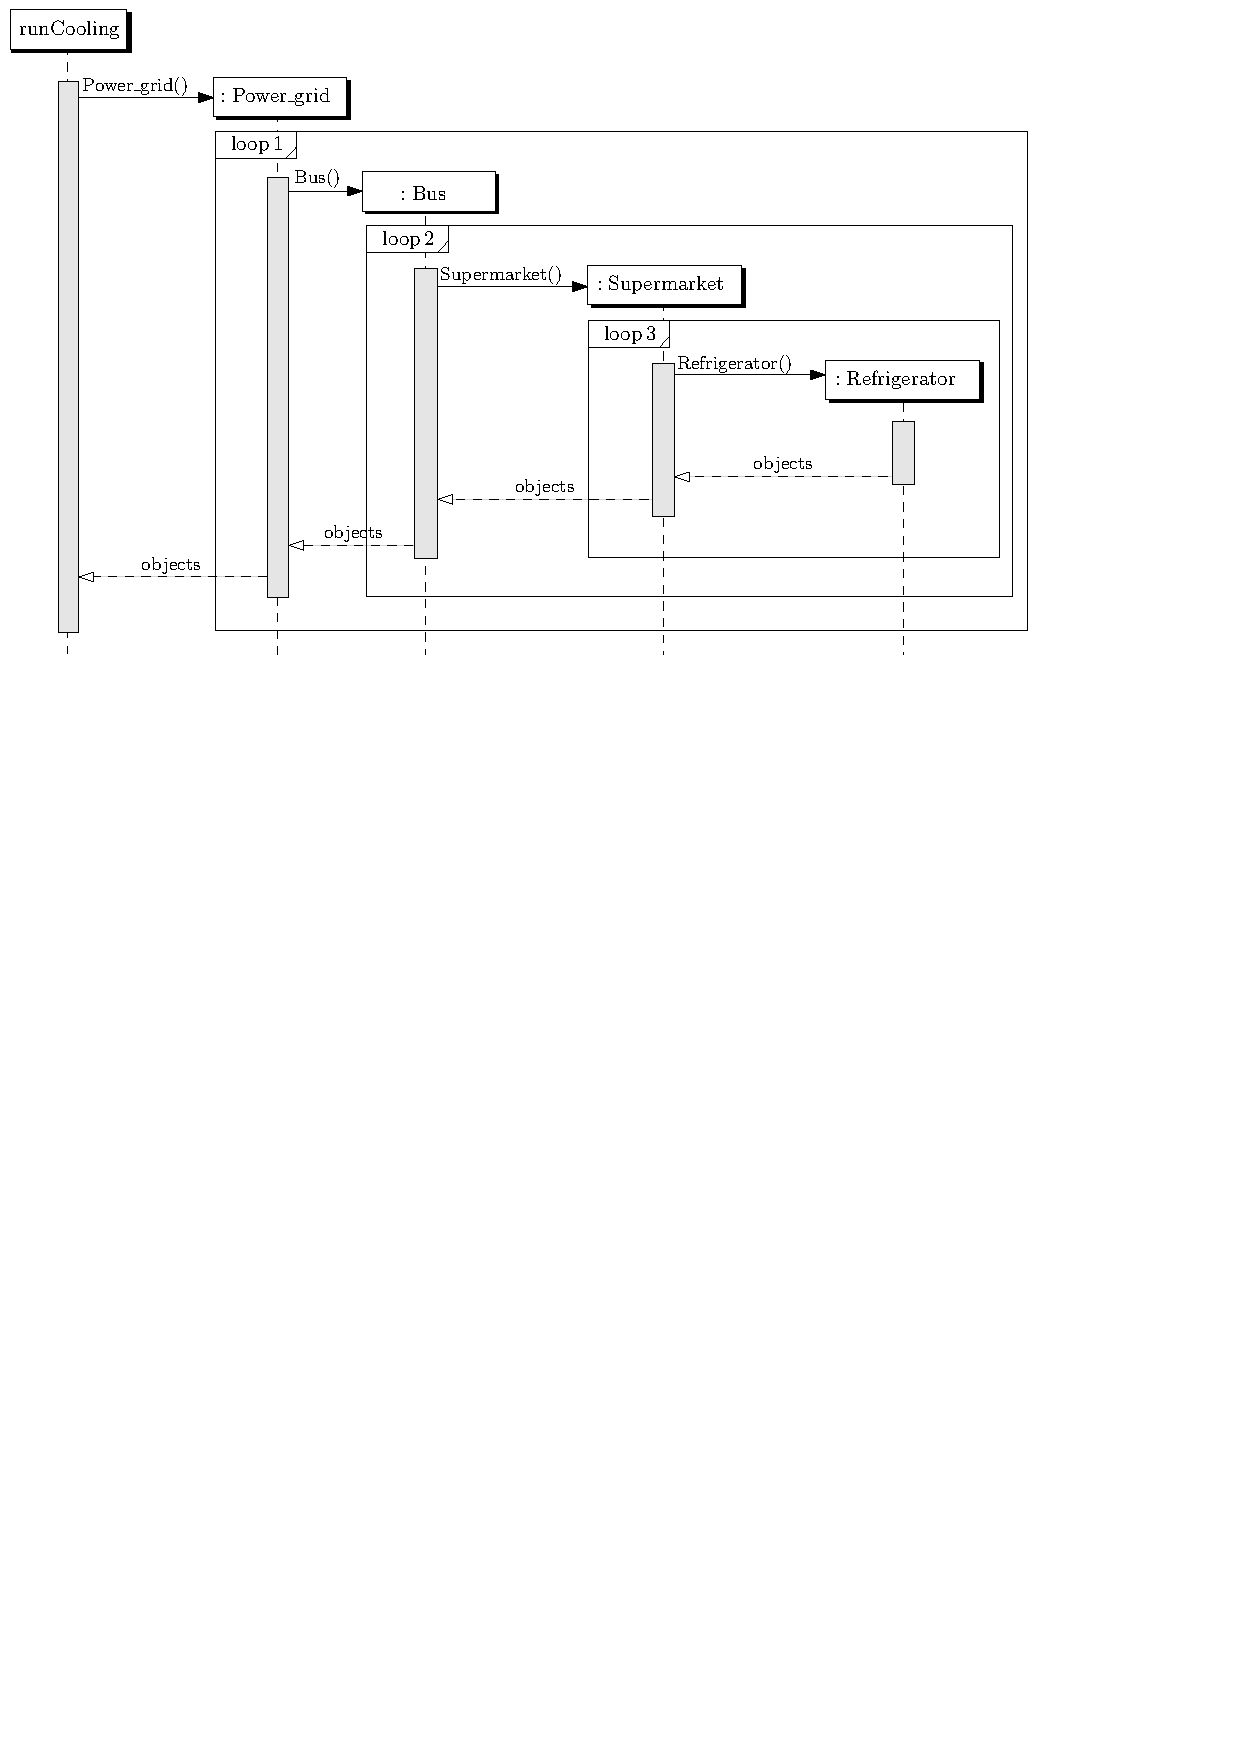
\includegraphics[scale=0.8]{images/Theorie_Super/sequence_one}
	\end{center}
\end{figure}

%%%%%%%%%%%%%%%%%%%%%%%%%%%%%%%%%%%%%%%%%%%%%%%%%%%%%%%%%%%%%%%%%%%%%%%%%%%%%%%%
%%%%%%%%%%%%%%%%%%%%%%%%%%%%%%%%%%%%%%%%%%%%%%%%%%%%%%%%%%%%%%%%%%%%%%%%%%%%%%%%

\section{Überblick über die mathematische Zusammenhänge}

In diesem Kapitel wird ein knapper \"Uberblick über die mathematischen und
physikalischen Zusammenhänge, die bei der Entwicklung eines Modellsupermarktes
zwingend beachtet werden müssen, vorgestellt\todo{Der Satz ist total scheiße
man}.

Die primäre Aufgabe der Kühleinheiten in einem Supermarkt besteht in der Regel
darin, Lebensmitteltemperatur unter die Zimmertemperatur zu bringen und diese
dabei zu halten\todo{Hört sich komisch an!}. Körper mit unterschiedlicher
Temperatur sind bestrebt, wenn sie thermisch von einander nicht vollkommen
isoliert sind, durch gegenseitige Wechselwirkung ihre Temperaturen anzugleichen,
sodass ein Wärmegleichgewicht entsteht, wobei der natürliche, selbständige
Wärmefluss immer von einem Körper mit höheren Temperatur in Richtung des Körpers
mit kleineren Temperatur stattfindet. Um eine negative Temperaturänderung
herzustellen und diese auch zu halten, muss die eindringende Wärmeenergie
ständig in der selben Höhe abgeführt werden, damit die Temperatur konstant
bleibt. Diese Energiemenge pro Zeiteinheit wird als Kälteleistung bezeichnet.
Eine Abweichung von dieser Menge führt zum Steigen der Temperatur, wenn weniger
und zum sinken der Temperatur wenn mehr abgeführt wird. Um diesen Kühlkreislauf
aufrecht zu erhalten, muss Leistung aufgewendet werden\footnote{ Eine
detailierte Beschreibung dieser Prozesse in einer Kopressionskälteanlage und
Spezifikation ist nicht Gegenstand dieser Arbeit.  Ausführliche Informationen
dazu findet man z.B.  in \cite{caro, doctor, TAB_A1}.}.

Das wird ausformuliert und mit einem Bild visualisiert\todo{bald schnell
machen}.
\begin{itemize}
	\item Temperaturunterschied in Kelvin $K$
	\item Wärmeausgleich (Verlust an Kälte)
	\item Kälteenergie gespeichert in Körpern mit einer bestimmten
	spezifischen Wärmekapazität
	\item Kälteenergie gespeichert in Masse
\end{itemize}
\begin{figure}\caption{ Modellgrundlage}
	\missingfigure{Modellgrundlage}
\end{figure}

Aufnahme der Wärmeenergie und der spezifischen Wärmekapazität dieser
Substanzmasse ergibt die Temperaturdifferenz $\Delta\:t$.

\begin{equation}
	\Delta\:t = \frac{Q}{m\cdot c}
\label{tdif}
\end{equation}

\begin{description}[\dth]

	\item[$\Delta\:t$] Temperaturdifferenz in Kelvin $K$
	\item[$Q$] Eindringende Wärmeenergie in $kJ$
	\item[$m$] Substanzmasse zur Aufnahme der Wärmeenergie in $kg$
	\item[$c$] Spezifische Wärmekapazität der Substanzmasse in $\frac{kJ}{kg
		\cdot K}$

\end{description}
\vspace{0.5cm}

Die installierte Kälteleistung multipliziert mit der täglichen Betriebszeit muss
zwangsweise größer oder gleich dem stündlichen Kältebedarf multipliziert mit der
Tagesstundenzahl sein.

\begin{equation}
	\pinstall = \frac{24\,h}{ \tau_{B} }  \cdot \pkalt \label{pinstall}
\end{equation}

\begin{description}[\dth]

	\item[$\pinstall$] Installierte Kälteleistung in $kW$
	\item[$\tau_{B}$] Tägliche Betriebszeit in $h$
	\item[$\pkalt$] Kältebedarf in $kW$

\end{description}
\vspace{0.5cm}

Die Transmissionswärmeleistung wird aus der Multiplikation der Fläche
der wärmeübertragenden Wänd mit ihrem spezifischen Wärmedurchgangskoeffizient
und der Temperaturdifferenz zwischen der Kühlraumtemperatur und der
Umgebungstemperatur berechnet.

\begin{equation}
	\ptrans = A \cdot k \cdot \Delta t
	\label{ptrans}
\end{equation}

\begin{description}[\dth]

	\item[$\ptrans$] Transmissionswärmeleistung in $kW$
	\item[$A$] Fläche in $m^2$
	\item[$k$] Wärmedurchgangskoeffiziente in $\frac{W}{m^2 \cdot K}$
	\item[$\Delta\: t$] Temperaturdifferenz in $K$

\end{description}
\vspace{0.5cm}

Der Zusammenhang zwischen der aufgewendeten elektrischen Antriebsleistung $P$
eines Verdichters in einer Kompressionskälteanlage und der genutzten
Kälteleistung ${\dot{Q}}_0$ wird durch die Kältezahl $\epsilon$ wiedergegeben.
Die Leistungszahl wird in die zweite Spalte im Array (vergl. Zeile 4 im
\matref{fridge}) eingetragen.

\begin{equation}
	\epsilon = \frac{\pkalt}{P}
\label{epsilon}
\end{equation}

\begin{description}[\dth]

	\item[$\epsilon$] Leistungszahl (einheitenlos)
	\item[$\pkalt$] Kälteleistungsbedarf in $kW$
	\item[$P$] elektrische Verdichterantriebsleistung in einer
		Kopressionskälteanlage in $kW$

\end{description}
\vspace{0.5cm}

Die Öffnungszeit des Supermarkts hat einen spürbaren Einfluss auf die Größe der
Wärmeverluste. In der Literatur wird der Nachtverbrauch mit $10\%$ bis $20\%$
des Tagesverbrauchs angegeben\cite{kauffeld}.  In der Nacht fallen keine
zusätzlichen Verluste zum Beispiel durch Licht, Körperwärme oder
Türöffnungszeiten, sodass nur Transmissionsverluste bei der Berechnung beachtet
werden.

\begin{equation}
	\dot{Q}_{Nacht}=\ptrans
\label{pnacht}
\end{equation}

\begin{description}[\dth]

	\item[$\pnacht$] Leistungsbedarf in der Nacht in $kW$
	\item[$\ptrans$] Transmissionswärmeleistung in $kW$

\end{description}
\vspace{0.5cm}


Der Leistungsbedarf am Tag ergibt sich aus der Summe des Tagesmehrbedarfs und
der Transmissionswärmeleistung. Aus Gründen der Vereinfachung wird
Tagesmehrbedarf als weitgehend konstant angenommen.

\begin{equation}
	\ptag = \pmehr + \ptrans
\label{ptag}
\end{equation}

\begin{description}[\dth]

	\item[$\ptag$] Leistungsbedarf am Tag in $kW$
	\item[$\pmehr$] Mehrbedarf am Tag in $kW$
	\item[$\ptrans$] Transmissionswärmeleistung in $kW$

\end{description}
\vspace{0.5cm}

Die Berechnung der mittleren Transmissionswärmeleistung erfolgt durch die
Multiplikation der Differenz zwischen der Umgebungstemperatur und der mittleren
Kühlraumtemperatur mit dem Wärmedurchgangskoeffizienten und der Fläche der
wärmeübertragenden Wände.

\begin{equation}
	\aptrans = A \cdot k \cdot \left( t_{amb} -
	\overline{t}_{KR} \right) \label{aptrans}
\end{equation}

\begin{description}[\dth]

	\item[$\aptrans$] mittlere Transmissionswärmeleistung in $kW$
	\item[$A$] Fläche in $m^2$
	\item[$k$] Wärmedurchgangskoeffiziente in $\frac{W}{m^2 \cdot K}$
	\item[$t_{amb}$] Umbgebungstemperatur in $^{\circ}C$
	\item[$\overline{t}_{KR}$] mittlere Kühlraumtemperatur in
		$^{\circ}C$
\end{description}
\vspace{0.5cm}

Ist f\"ur eine K\"alteanlage der K\"alteleistungsbedarf bekannt so wird der
Tagesmehrbedarf an K\"alteleistung ermittelt, indem vom Produkt des
K\"alteleistungsbarfes f\"ur $24\;h$ mit dem Faktor f\"ur
K\"altebedarfsabsenkung die mittlere Transmissionswärmeleistung abgezogen wird.

\begin{equation}
	\pmehr = \pkalt \cdot K - \aptrans
\label{pmehr}
\end{equation}

\begin{description}[\dth]

	\item[$\pmehr$] Mehrbedarf am Tag in $kW$
	\item[$\pkalt$] Kälteleistungsbedarf in $kW$
	\item[$K$] Faktor für Kältebedarfsabsenkung (einheitenlos)
	\item[$\aptrans$] mittlere Transmissionswärmeleistung in $kW$

\end{description}
\vspace{0.5cm}

Ist der Kälteleistungsbedarf nicht bekannt, wie zum Beispiel bei steckerfertigen
Geräten, kann der Mehrbedarf am Tag \"uber den Wert Verdichterarbeit pro 24
Stunden $\lverd$ für den gesamten Kälteverbraucher ermittelt werden.

Das Produkt aus dem spezifischen Energieverbrauch mit dem Faktor für
Kältebedarfsabsenkung, dem Verdichteranteil und der Anzahl der Geräte ergibt die
Verdichterarbeit.

\begin{equation}
	\lverd = \lspez \cdot K \cdot v \cdot n
\label{lverd}
\end{equation}

\begin{description}[\dth]

	\item[$\lverd$] Verdichterarbeit pro $24\,h$ in $\frac{kWh}{24h}$
	\item[$\lspez$] spezifischer Energieverbrauch pro $24\,h$ in
		$\frac{kWh}{24h}$
	\item[$K$] Faktor für Kältebedarfsabsenkung (einheitenlos)
	\item[$v$] Verdichteranteil (einheitenlos)
	\item[$n$] Anzahl der Geräte

\end{description}
\vspace{0.5cm}

Im Folgenden muss die Verdichterarbeit zum Abf\"uhren von zus\"atzlich
eindringenden W\"aremeenergie in der \"Offnungszeit berechnet werden, die einem
weiteren Schritt in W\"armeleistung $\pmehr$ umgewandelt wird.

\begin{equation}
	\lmehr = \lverd - \frac{\ptrans}{\epsilon} \cdot 24h
\label{lmehr}
\end{equation}

\begin{description}[\dth]

	\item[$\lmehr$] Verdichterarbeit zum Abführen von eindringenden
		Wärmeenergie $\emehr$ in $kWh$ in der \"Offnungszeit
	\item[$\lverd$] Verdichterarbeit pro $24\,h$ in $\frac{kWh}{24h}$
	\item[$\ptrans$] Transmissionswärmeleistung in $kW$
	\item[$\epsilon$] Leistungszahl (einheitenlos)

\end{description}
\vspace{0.5cm}

Die Umrechnung von $\lmehr$ in $\pmehr$ erfolgt mit Hilfe der Leistungszahl
$\epsilon$. Die Verdichterarbeit $\lmehr$ wird mit $\epsilon$ multipliziert.
Es wird angenommen, dass der Mehrbedarf in den rund zw\"olf Stunden der
\"Offnungszeit einf\"a

\begin{equation}
	\pmehr = \frac{\lmehr}{12h} \cdot \epsilon
\label{<++>}
\end{equation}

\begin{description}[\dth]

	\item[$\pmehr$] Mehrbedarf am Tag in $kW$
	\item[$\lmehr$] Verdichterarbeit zum Abführen von eindringenden
		Wärmeenergie $\emehr$ in $kWh$ in der \"Offnungszeit
	\item[$\epsilon$] Leistungszahl (einheitenlos)

\end{description}
\vspace{0.5cm}
berechnen.

Dabei entspricht $\pnacht$ der mittleren Transmissionswärmeleistung $\ptrans$.
$\ptag$ ist der Kältebedarf $\pkalt$, multipliziert mit dem Faktor für die
Kältebedarfsabsenkung $K$ bei Geräten, bei denen der Kältebedarf gegeben ist.
Bei steckerfertigen Geräten ist $\ptag$ die Summe aus dem Mehrbedarf an Leistung
am Tag $\pmehr$ und der mittleren Transmissionswärmeleistung $\ptrans$.

Mit den Wärmeverlusten, die am Tag und in der Nacht in unterschiedlicher Größe
auftreten, wird für jeden Zeitschritt die Zeit bis zum kritischen
Temperaturmaximum bestimmt. Diese Zeit braucht das Programm, um den Einsatz der
Supermarktkälteanlagen als Speicher zu planen. Mit der Gleichung

\begin{equation}
	\tau_{krit}(i) = \frac{m \cdot c \cdot (t_{max} -
		t(i))}{\aptranslog}
\label{taukn}
\end{equation}

\begin{description}[\dth]

	\item[$\tau_{krit}$] Zeit bis zur kritischen Temperatur in $h$
	\item[$m$] Substanzmasse zur Aufnahme der Wärmeenergie in $kg$
	\item[$c$] Spezifische Wärmekapazität der Substanzmasse in $\frac{kJ}{kg
		\cdot K}$
	\item[$t_{max}$] obere Temperaturgrenze in $ ^{\circ} C $
	\item[$t(i)$] Temperatur zur Stunde $i$ in $ ^{\circ} C $
	\item[$\aptranslog$] logrithmierte Mittelwert der
		Transmissionswärmeleistung in $kW$|
\end{description}
\vspace{0.5cm}


wird die Zeit $\tau_{krit}$ für jeden Zeitpunkt $i$ berechnet, wobei
$\overline{\dot{Q}}_{Tr_{ln}}$ der logarithmische Mittelwert ist, der sich aus
den Transmissionswärmeleistungen zum jeweils aktuellen Zeitpunkt $i$ mit der
Temperatur $t(i)$ und den Transmissionswärmeleistungen zum Zeitpunkt, an dem der
Kühlinnenraum die maximale Temperatur $t_{max}$ erreicht hätte, berechnet. Am
Tag müssen die restlichen Verluste $\pmehr$ zusätzlich zu den
Transmissionwärmeverlusten für die Berechnung der Zeit bis zur kritischen
Temperatur berücksichtigt werden, wodurch sich folgende Gleichung ergibt:

\begin{equation}
	\tau_{krit}(i) = \frac{m \cdot c \cdot (t_{max} -
		t(i))}{{\overline{\dot{Q}}_{Tr_{ln}}} + \pmehr}
\label{taukd}
\end{equation}

\begin{description}[\dth]

	\item[$\tau_{krit}$] Zeit bis zur kritischen Temperatur in $h$
	\item[$m$] Substanzmasse zur Aufnahme der Wärmeenergie in $kg$
	\item[$c$] Spezifische Wärmekapazität der Substanzmasse in $\frac{kJ}{kg
		\cdot K}$
	\item[$t_{max}$] obere Temperaturgrenze in $ ^{\circ} C $
	\item[$t(i)$] Temperatur zur Stunde $i$ in $ ^{\circ} C $
	\item[$\aptranslog$] logrithmierte Mittelwert der
		Transmissionswärmeleistung in $kW$
	\item[$\pmehr$] Mehrbedarf am Tag in $kW$

\end{description}
\vspace{0.5cm}

Die Zeit $\tau_{krit}$ ist abhängig vom Anstieg der Temperaturen und dieser
wiederum von den eindringenden Wärmelasten.

Um den Temperaturausgleich in den Lebensmitteln im Algorithmus zu
berücksichtigen, werden deshalb die zu- und abgeführten Wärmeenergiemengen bei
der Berechnung der Temperatur für jeden Zeitschritt stets mit dem Faktor 0,8
multipliziert.  Die Gleichung zur stündlichen Berechnung der aktuellen
Temperatur ist damit:

\begin{equation}
	t(i+1) = 0.8 \cdot \frac{Q_v - Q_{ab}}{m \cdot c} + t(i)
\label{tns}
\end{equation}

\begin{description}[\dth]

	\item[$t$] Temperatur in $^{\circ} C$
	\item[$Q_v$] eindringende Verlustwärmemenge in $kJ$
	\item[$Q_{ab}$] abführende Wärmemenge in $kJ$

\end{description}
\vspace{0.5cm}

wobei $Q_v$ die aktuell eindringende Wärmeenergie und $Q_ab$ die abgeführte
Wärmeenergie ist.

% \chapter{Problemanalyse}
\label{chap:problemstellung}
\minitoc
%%%%%%%%%%%%%%%%%%%%%%%%%%%%%%%%%%%%%%%%%%%%%%%%%%%%%%%
%%%%%%%%%%%%%%%%%%%%%%%%%%%%%%%%%%%%%%%%%%%%%%%%%%%%%%%
%%%%%%%%%%%%%%%%%%%%%%%%%%%%%%%%%%%%%%%%%%%%%%%%%%%%%%%

In diesem Kapitel wird ein detailliertes Bild über die Aufgabenstellung gegeben. Außerdem werden die Schritte, die beim
Programmentwurf in der Planungsphase durchgegangen worden sind, Punkt für Punkt beschrieben.

\section{Aufgabenstellung}

Ein Programm zur Simulation des variablen Lastverhaltens von Kältelast mit Kältespeicher im
Energieversorgungsnetz\todo{Aufgabenstellung richtig beschreiben}.

\begin{itemize}
	\item Präzisierung
	\item Formalisierung
\end{itemize}

\begin{itemize}
	\item netzbezogene Beschränkungen
	\item kältetechnische Beschränkungen
\end{itemize}

Das Simulationsprogramm wird im Zusammenhang mit einem Lastflussoptimierungsprogramm aufgerufen.

\section{Erster Schritt der Planung}

Die an das Programm gestellten Anforderungen werden im ersten Schritt des Softwareentwurfs bestimmt. Die Ermittlung
der Funktionen des Programms, sowie die Form und die Menge der Daten, die in das Programm fließen müssen, bilden das Ziel der
ersten Phase der Planung.

\subsection{Funktionen und Daten}

Die Intention der Arbeit, ein Programm zur Simulation des variablen Lastverhaltens von Kältelast mit Kältespeicher im
Energieversorgungsnetz, bestimmt die Funktionen, die das Simulationsprogramm zu erfüllen hat. Dem Anwender des Programms wird
die Möglichkeit bereitgestellt, das Lastverhalten einer variablen Anzahl an Modellkältelasten in einem beliebigen
Energieversorgungsnetz in Folge vom Anwender bestimmten Lasmanagementes zu simulieren um anschließend die Verbrauchsdaten in
einem Lastflussoptimierungsprogramm zu verwenden.


Im Energieversorgungsnetz ist eine Kältelast ein gewöhnlicher Energieverbraucher, der an Knoten des Energieversorgungsnetzes
angeschlossen ist. Besonderes interessant als Untersuchungsgegenstand bei der Betrachtung der Möglichkeiten zum Lastmamagement
im Ramen der Integration der fluktuierenden Erneuerbaren Energie in ein Energieversorgungsnetz wird diese Art der Last,
speziell die Kälteanlagen in den bestehenden Supermarktketten, durch die Tatsache, dass einen hoher Prozentanteil am
Gesamtenergieverbrauch eines Landes darauf abfällt \cite{doctor}\todo{freaky}. Der durchschnittliche Energieverbrauch der
Kälteanlagen je Supermaktkette kann auf Grund der technischen Ausführung unterschiedlich sein. Der Energieverbrauch entsteht
also an definierten Punkten im Netz. An den einzelnen Knotenpunkten können mehrere Kältelasten angeschlossen sein.

Auf Grund dieser Analyse erscheinen folgende Funktionen für die Umsetzung des Programms besonders zweckmäßig.

\begin{itemize}
	\item Eines auf das Problem reduziertes Computermodell des Energieversorgungsnetzes wird erstellt. Die relevanten
	Input-Informationen sind:
	\begin{itemize}
		\item Anzahl der Knoten,
		\item Anzahl der an einen Knoten angeschlossene Speicher,
		\item Menge der zu regelnder Energie,
		\item bzw. LMP-Preise.
	\end{itemize}
	\item Ein Computermodell der Kältelast wird erstellt. Die relevanten Input-Informationen sind:
	\begin{itemize}
		\item Modellparameter Kältelast.
	\end{itemize}
	\item Der Informationsfluss zwischen den Computermodellen Energieversorgungsnetz und Kältelast wird in einer Weise
	implementiert, die es ermöglicht, den elektrischen Energieverbrauch der jeweiligen Kältelasten eindeutig zu berechnen
	und dem Verursacher sowie dem Anschlussort, an dem die Energie verbraucht wird, zuzuordnen. Der elektrische
	Energieverbrauch wird auf Grund der Modellparameter der Kältelasten sowie 
\end{itemize}


% \chapter{Problemspezifikation: Ermittlung eines Lösungwegs}
\label{chap:problemspezifikation}
\minitoc
%%%%%%%%%%%%%%%%%%%%%%%%%%%%%%%%%%%%%%%%%%%%%%%%%%%%%%%
%%%%%%%%%%%%%%%%%%%%%%%%%%%%%%%%%%%%%%%%%%%%%%%%%%%%%%%
%%%%%%%%%%%%%%%%%%%%%%%%%%%%%%%%%%%%%%%%%%%%%%%%%%%%%%%
\begin{itemize}
\item Ermitteln eines Lösungsweges
\end{itemize}
In diesem Kapitel wird anhand eines vier Knoten Beispielnetzes vorgestellt, Lösung Problem\todo{Der Einführungsabsatz ist zu
schreiben.}. Unabhängig von dem mathematischen Modell des Modellsupermarktes wird die Umsetzung der Implementierung
vorgestellt\todo{Was ist los?}.

\section{Problemlösungsansatz}

OOP\abvz{OOP}{objektorientierte Programmierung}: Lösung von Problemen durch ein Gefecht kooperierender Objekte.\cite{java}
%%%%%%%%%%%%%%%%%%%%%%%%%%%%%%%%%%%%%%%%%%%%%%%%%%%%%%%
%%%%%%%%%%%%%%%%%%%%%%%%%%%%%%%%%%%%%%%%%%%%%%%%%%%%%%%
%%%%%%%%%%%%%%%%%%%%%%%%%%%%%%%%%%%%%%%%%%%%%%%%%%%%%%%
\subsubsection*{Gedankliche Konzepte, Motivation und Einsatz der OOP}
Seit Ende des letzten Jahrhunderts herrscht in der Fachliteratur für Informatik die Meinung, dass der Einsatz von
objektorientierten Techniken beim Softwareentwurf Programme hervorbringt, die im Vergleich \textit{einfacher erweiterbar,
besser testbar} und \textit{besser wartbar} sind\todo{SIND, das ist hier nicht gut.}. Dabei wird ein Verfahren angewendet, nach
dem große Systeme in kleinere Teile des Ganzen zerlegt werden. Diese lassen sich dann im Allgemeinen mit weniger Aufwand und
Fehlerwahrscheinlichkeit programmieren. Inspiriert durch die Vorgänge aus der realen Welt, werden die Abläufe durch
operierende Objekte vorgestellt, die Aufträge erledigen und vergeben können.  Die obengenannte Aufgabenstellung und die
Thematik erlaubt es mit Hilfe der Grundelemente der objektorientierten Software\todo{Was ist hier mit dem Komma?},
\textit{Datenkapselung, Polymorphie <<Vielgestaltigkeit>> und Vererbung}, die Lösung des Problems mit Zuversicht anzugehen
und ein flexibles Programm herzustellen. Es besteht die Möglichkeit, Supermarktketten mit unterschiedlicher Ausführung, Größe
und unterschiedlichem Energieverbrauch in einem Energieversorgungsnetz flexibel zu modellieren\footnote{ Ausführliche
Informationen dazu findet man z.B. in \cite{OOP},\cite{java} oder \cite{python}.}\todo{Das ist nicht ganz ok?}.


%%%%%%%%%%%%%%%%%%%%%%%%%%%%%%%%%%%%%%%%%%%%%%%%%%%%%%%
%%%%%%%%%%%%%%%%%%%%%%%%%%%%%%%%%%%%%%%%%%%%%%%%%%%%%%%
%%%%%%%%%%%%%%%%%%%%%%%%%%%%%%%%%%%%%%%%%%%%%%%%%%%%%%%



\section{Anwendung der OOP am Modell}
In der \cref{vkb} wird ein einfaches Energieversorgungsnetz mit vier Knoten dargestellt. Am Knoten eins ist eine regenerative
elektrische Energiequelle, in diesem Fall ein Windpark, angeschlossen. Weitere konventionelle elektrische Energiequellen
befinden sich an den Knoten zwei und drei. Die passiven Lasten befinden sich am Knoten zwei und vier. Der Kältespeicher ist am
Knoten zwei angeschlossen. Im Bild wird der Kältespeicher Supermarkt durch einen Einkaufswagen symbolisiert. Die Knoten sind
untereinander durch Leitungen verbunden.

\begin{figure}[h]
\caption{Vier Knoten Beispiel}
	\label{vkb}
	\begin{center}
	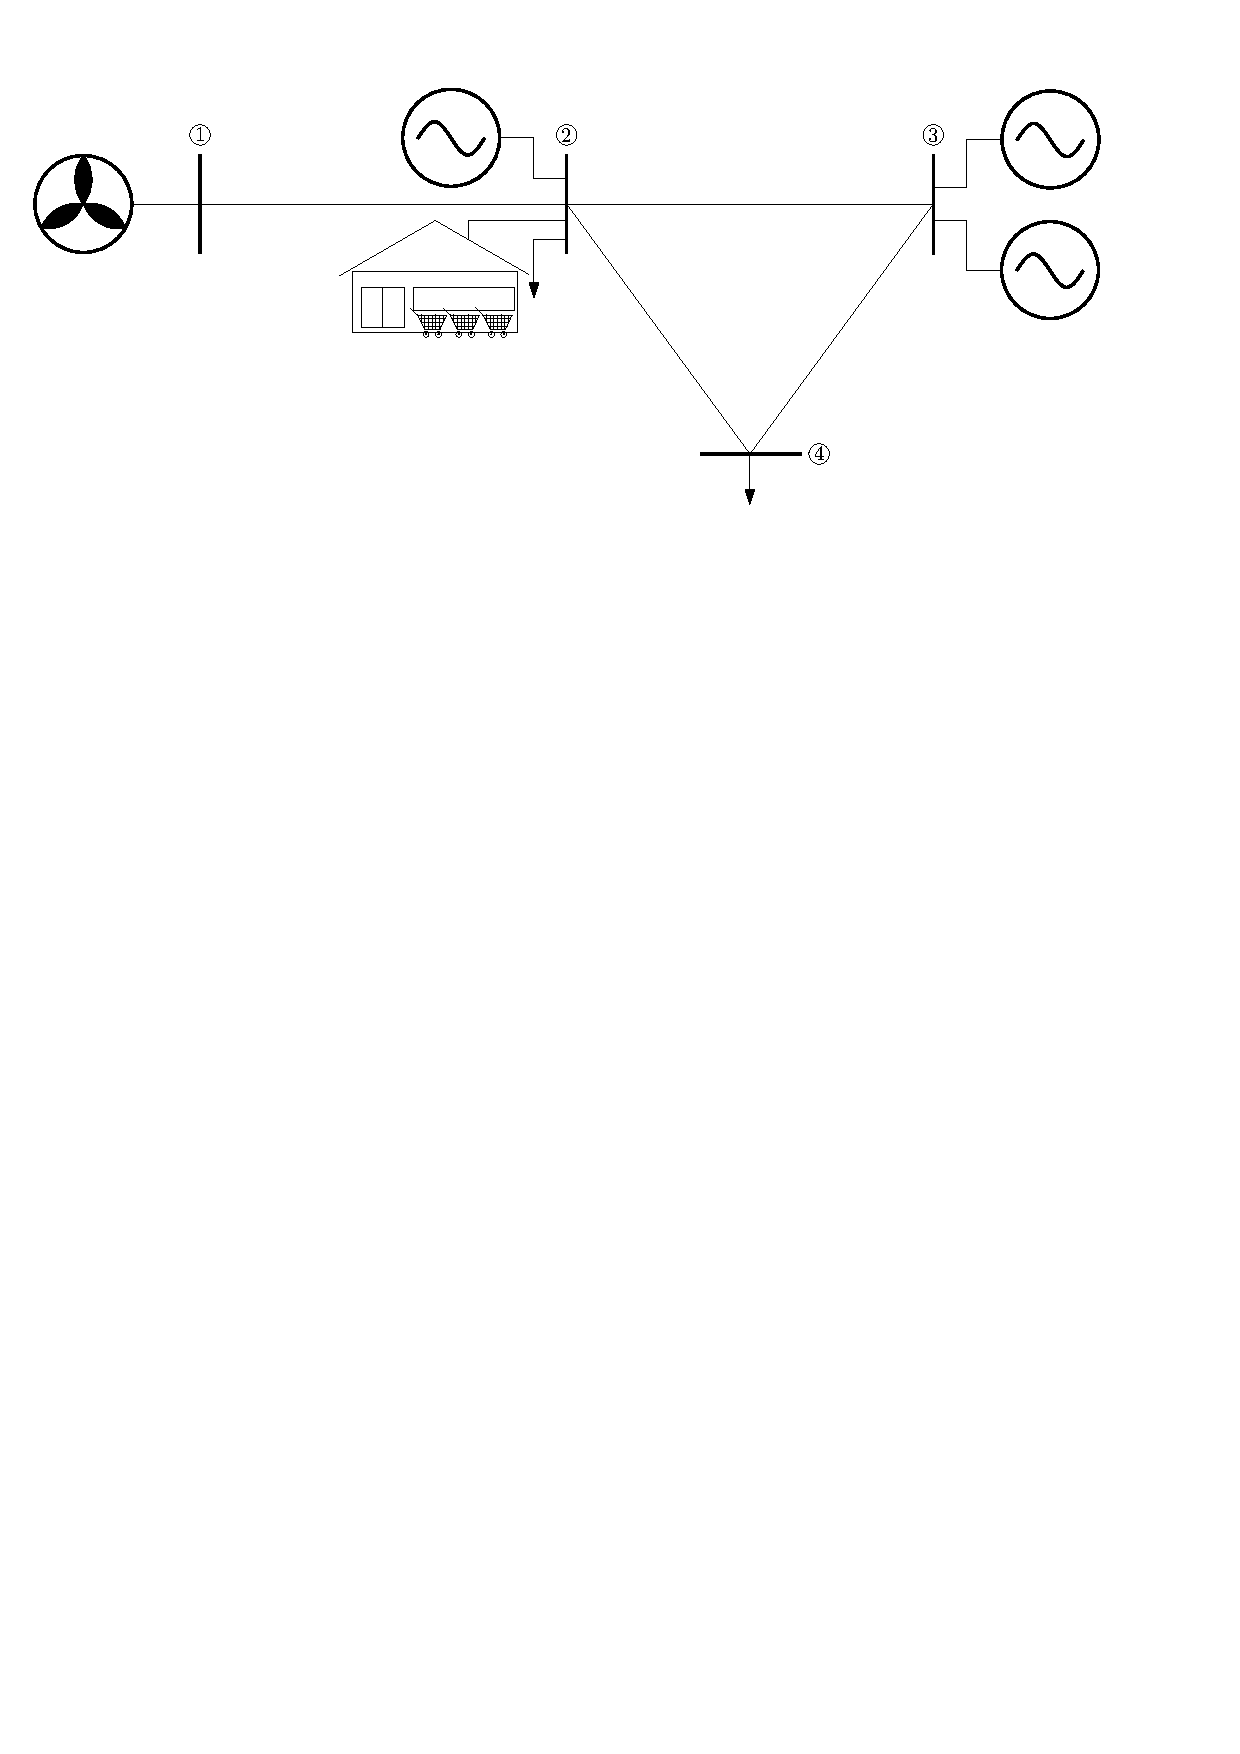
\includegraphics[scale=0.75]{images/SEVN/power_grid}
	\end{center}
\end{figure}

In der Realität kann ein Energieversorgungsnetz durch die Variation der Knotenzahl und die Vermaschung beliebig komplizierte
Form aufweisen. Bei der Umsetzung der gegebenen Situation im Programm.

\begin{figure}[h]
\caption{Klassendiagramm Modellkonstrukt}
	\label{klassendiagramm}
	\begin{center}
	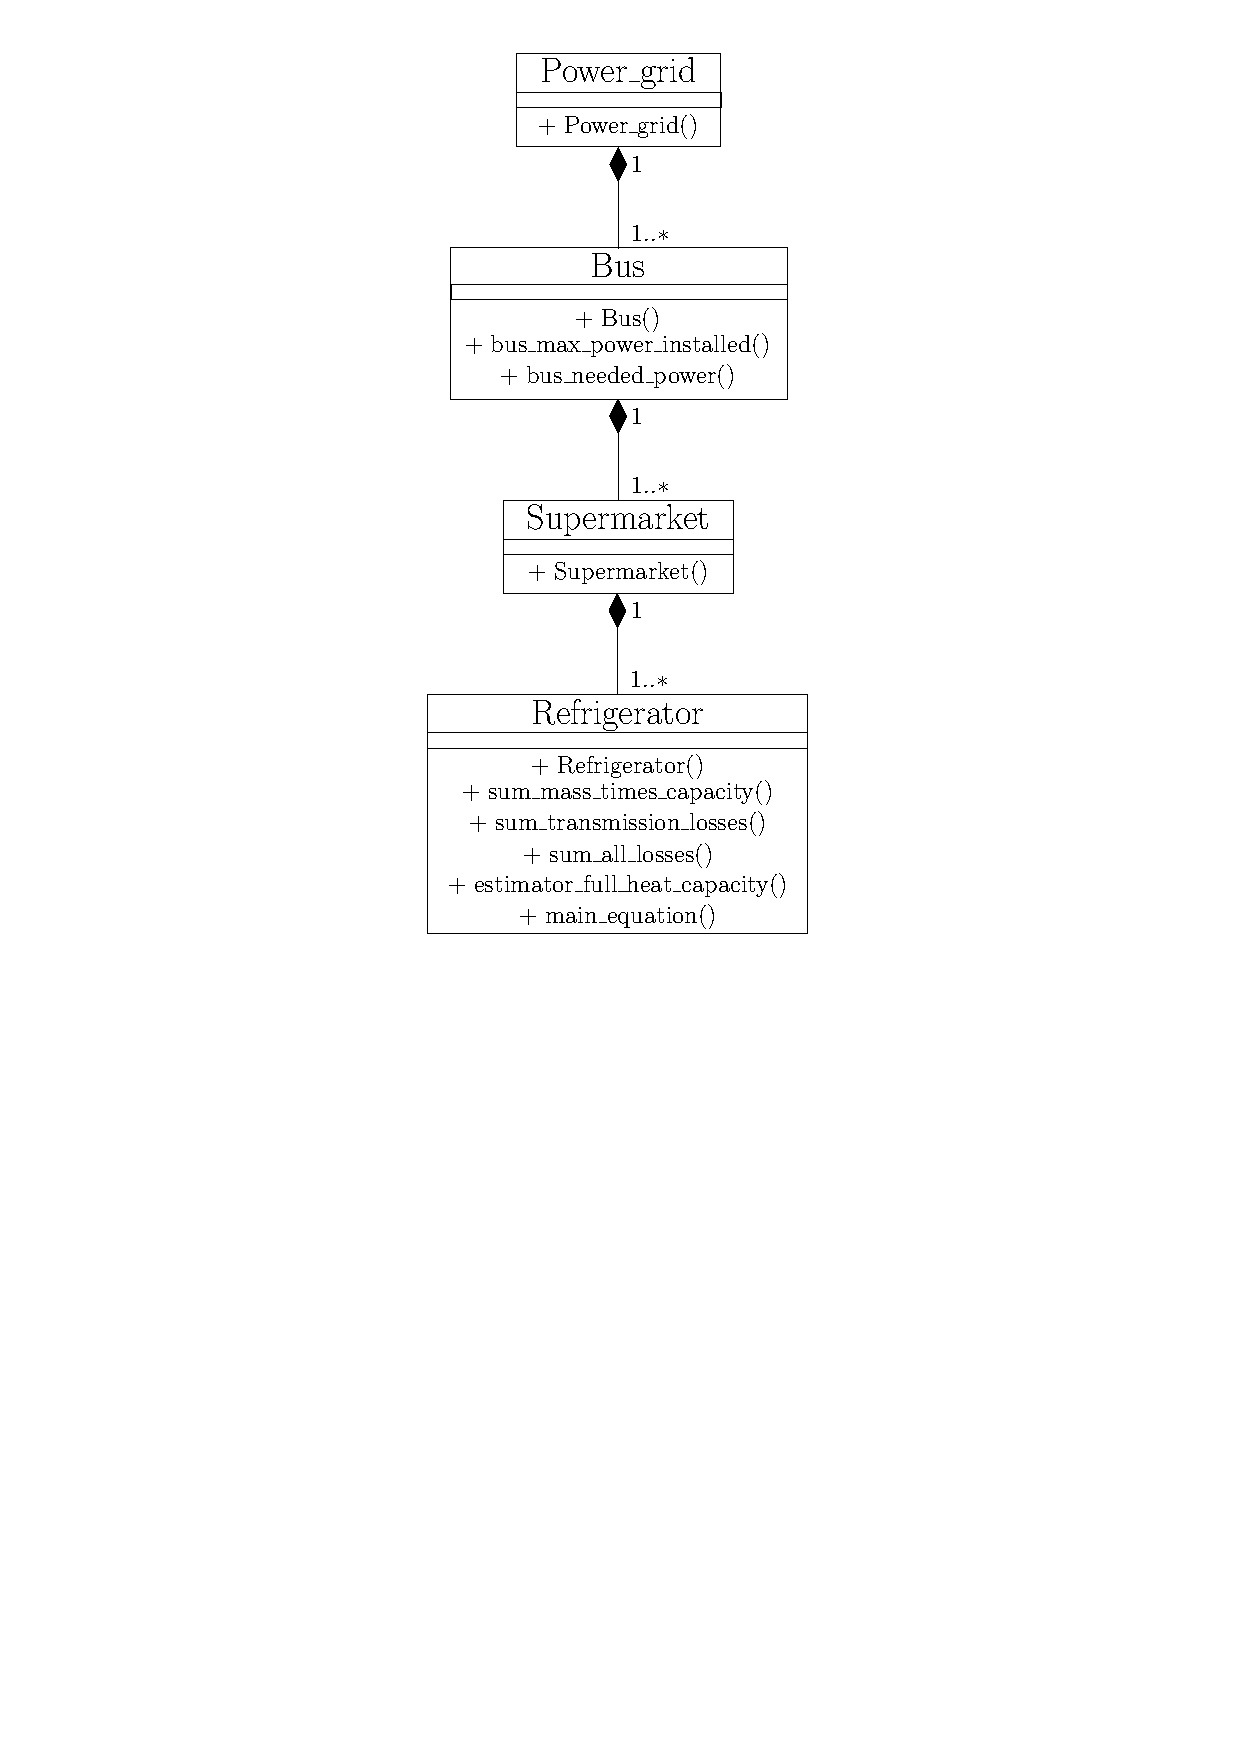
\includegraphics[scale=0.8]{images/Theorie_Super/class_diagramm}
	\end{center}
\end{figure}

Hier noch ein Zwischentext.

\begin{figure}[h]
\caption{Sequenzdiagramm Modellkonstrukt}
	\label{uml_sequence}
	\begin{center}
	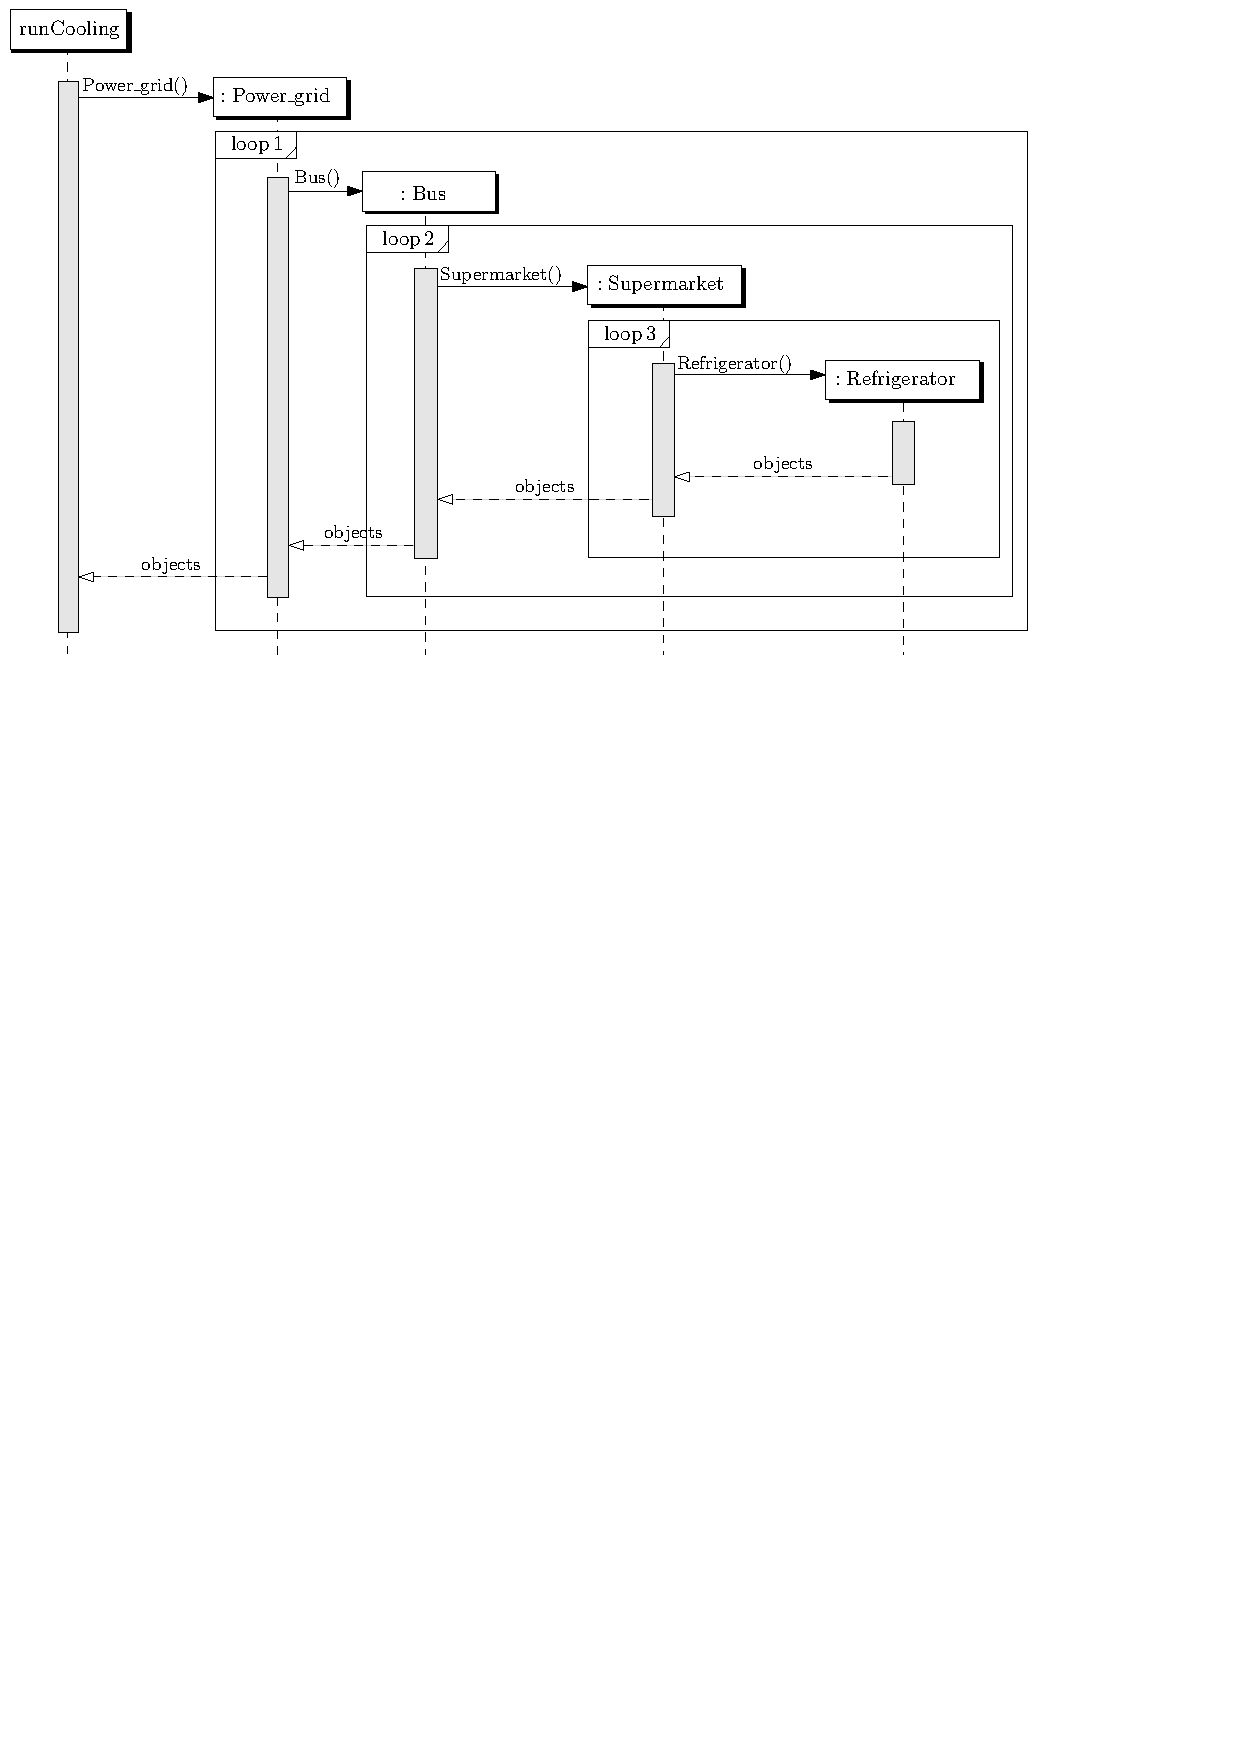
\includegraphics[scale=0.8]{images/Theorie_Super/sequence_one}
	\end{center}
\end{figure}


% \include{Konkretisierung_Lousungsweg}
% \chapter{Handhabung des Programms}
\label{chap:handhabung}
\minitoc

%%%%%%%%%%%%%%%%%%%%%%%%%%%%%%%%%%%%%%%%%%%%%%%%%%%%%%%%
%%%%%%%%%%%%%%%%%%%%%%%%%%%%%%%%%%%%%%%%%%%%%%%%%%%%%%%%
%%%%%%%%%%%%%%%%%%%%%%%%%%%%%%%%%%%%%%%%%%%%%%%%%%%%%%%%
\section{Allgemeines}

Das Programm ist ein Packet aus \matlab M-files zur Simulation von Kälteanlagen mit Kältespeichern\footnote{ Da gewöhnliche
Supermarktketten Untersuchungsobjekt dieser Studie sind, werden die Termini Kältelast, Kälteanlagen mit Kältespeichern und
Supermarktkette als gleichbedeutend aufgefasst und verwendet.} in einem Energieversorgungsnetz. Das Simulationsprogramm ist
in der Lage das Verhalten einer bzw. mehrerer Supermarktkälteanlagen als flexibler Verbraucher in einem
Energieversorgungsnetz zu simulieren. Das Programm kann über eine vordefinierte Schnittstelle in ein
Leistungsflussberechnungs-Programm eingebunden werden.

%%%%%%%%%%%%%%%%%%%%%%%%%%%%%%%%%%%%%%%%%%%%%%%%%%%%%%%%
%%%%%%%%%%%%%%%%%%%%%%%%%%%%%%%%%%%%%%%%%%%%%%%%%%%%%%%%
%%%%%%%%%%%%%%%%%%%%%%%%%%%%%%%%%%%%%%%%%%%%%%%%%%%%%%%%
\subsection{Systemanforderungen}

Zur Benutzung des Programms muss auf Grund der gewählten Programmiersprache und der objektorientierten Programmierwiese
folgendes gelten:

\begin{itemize}
	\item Im Rechner muss die Software \matlab der Version $5.0$ oder höher\footnote{ \matlab verfügbar über The
		MathWorks, Inc.  (http://www.mathworks.com).} eingerichtet sein.
\end{itemize}

Die Anforderungen an die Hardware sind durch die eingesetzte \matlab-Version bestimmt.

%%%%%%%%%%%%%%%%%%%%%%%%%%%%%%%%%%%%%%%%%%%%%%%%%%%%%%%%
%%%%%%%%%%%%%%%%%%%%%%%%%%%%%%%%%%%%%%%%%%%%%%%%%%%%%%%%
%%%%%%%%%%%%%%%%%%%%%%%%%%%%%%%%%%%%%%%%%%%%%%%%%%%%%%%%
\subsection{Installation}

Das Programm richtet sich in seiner Installation und der Benutzung nach dem allgemein gültigen Gebrauch der \matlab
M-files\footnoteremember{matlab}{ Ausführliche Information dazu findet man z.B. im \cite{MATLAB-Buch}.}.

%%%%%%%%%%%%%%%%%%%%%%%%%%%%%%%%%%%%%%%%%%%%%%%%%%%%%%%%
%%%%%%%%%%%%%%%%%%%%%%%%%%%%%%%%%%%%%%%%%%%%%%%%%%%%%%%%
%%%%%%%%%%%%%%%%%%%%%%%%%%%%%%%%%%%%%%%%%%%%%%%%%%%%%%%%
\subsection{Aufruf der Simulation}%

Die Primärfunktion des Programms ist, wie oben schon erwähnt, die Simulation des Lastverhaltens eines Supermarkts oder
mehreren Supermarktketten in einem Energieversorgungsnetz. Das setzt voraus, dass folgende grundlegende Prinzipien realisiert
werden:
\begin{enumerate}
	\item Ein oder mehrere \matlab-Modelle von Supermärkten können erstellt und gleichzeitig an verschiedenen Knoten im
		Energieversorgungsnetz verwendet werden.
	\item Von einem besonderen Interesse sind die Energieverbrauchszahlen zum Beispiel für einen bestimmte Kälteeinheit
		oder für die gesamte Kette. Die Realisierung der Speicherung dieser Daten ist zwingend.
\end{enumerate}

%%%%%%%%%%%%%%%%%%%%%%%%%%%%%%%%%%%%%%%%%%%%%%%%%%%%%%%%
%%%%%%%%%%%%%%%%%%%%%%%%%%%%%%%%%%%%%%%%%%%%%%%%%%%%%%%%
%%%%%%%%%%%%%%%%%%%%%%%%%%%%%%%%%%%%%%%%%%%%%%%%%%%%%%%%
\subsubsection{Vorbereitung der Input-Information}
\label{sec:input_infos}

Je nach Fall oder theoretischer Grundlage können die Konfigurationsdateien verändert werden\todo{das ist scheiße!}.
Zum Starten des Programms werden folgende Konfigurationsdateien benötigt:

\begin{itemize}
	\item config\_grid.m
	\item config\_supermarkets.m
	\item config\_fridges.m
\end{itemize}
%%%%%%%%%%%%%%%%%%%%%%%%%%%%%%%%%%%%%%%%%%%%%%%%%%%%%%%%
%%%%%%%%%%%%%%%%%%%%%%%%%%%%%%%%%%%%%%%%%%%%%%%%%%%%%%%%
%%%%%%%%%%%%%%%%%%%%%%%%%%%%%%%%%%%%%%%%%%%%%%%%%%%%%%%%
\vspace{3mm}
\noindent\textbf{config\_grid.m}
\vspace{3mm}

Es ist wichtig, dass die topologische Eigenschaft des Netzes im Programm berücksichtigt werden, damit bei der
Berechnung des Leistungsflusses die Laständerung, die durch den Betrieb der Kältelast entsteht, am Knoten, an dem sie
verursacht wird, gezählt wird\todo{freaky sentence}. Damit das Programm mit den für die Simulation notwendigen Informationen,
die das Energienetz beschreiben, versorgt wird, ist die Form, die in \matref{cgrid} vorgestellt wird, für die
\textbf{config\_grid.m$\,$}-Datei zwingend:

\begin{lstlisting}[float=h,caption={config\_grid.m},label={cgrid}]
%%	Bus,  Supermarkets,	  Number of Supermarkets
configuration_grid = {...
        1 , {Aldi	     ,	      1500;	     ...
             Netto	     ,	       500};	 ...
        2 , {0	         ,           0};	 ...
        3 , {0	         ,           0};	 ...
        4 , {0	         ,           0}	     ...
       };
\end{lstlisting}

In der \textbf{config\_grid.m}$\,$-Datei wird  ein $n\times2\,$-Cell Array ($n\in \mathbb{Z}^+_0$) definiert, der die
Information über die Topologie des Netzes sowie die Verteilung der Kältelasten im Netz beinhaltet. Ein Cell Array ist ein
Speicherobjekt, der verschiedene Datentypen unterschiedlicher Größe aufnehmen kann\cite[Teil 2, Seite 15]{MATLAB-Buch}.  Ein
Cell Array wird mit dem Befehl $c=cell(\ldots)$ oder mit Hilfe von geschweiften Klammern $c=\{\ldots\}$, wie in diesem Fall,
erzeugt. Der Zugriff auf ein Cell Array wird in dem folgenden Kapitel\todo{Hier auf Kapitel verweisen.}$\,$ kurz
erklärt\footnoterecall{matlab}. Jede Zeile des Cell Arrays \textbf{configuration\_grid}, der in der
\textbf{config\_grid.m}$\,$-Datei definiert werden muss, steht für ein Knotenpunkt im Netz. In der ersten Spalte wird die
Nummer des Knotens bzw. Busses gespeichert. In die zweite Spalte werden die Arten der Kältelasten und deren Anzahl an
jeweiligen Knoten festgelegt. Es ist wiederum ein $m\times2\,$-Cell Array ($m\in \mathbb{Z}^+_0$). Jede Zeile dieses Cell
Arrays ist für eine eigene Art Supermarktkette reserviert. In die erste Spalte kommt der Name der Supermarktkette deren
Eigenschaften in der \textbf{config\_supermarkets.m$\,$}-Datei vergl.  \matref{csuper} gespeichert sind. In die zweite Spalte
wird die Anzahl der Supermärkte einer Kette festgelegt die an dem bestimmten Knoten simuliert werden soll.

Um Fehler auf dieser Ebene zu vermeiden, muss die \textbf{config\_grid.m}$\,$-Datei unbedingt die oben vorgestellte Form
beibehalten.

%%%%%%%%%%%%%%%%%%%%%%%%%%%%%%%%%%%%%%%%%%%%%%%%%%%%%%%%
%%%%%%%%%%%%%%%%%%%%%%%%%%%%%%%%%%%%%%%%%%%%%%%%%%%%%%%%
%%%%%%%%%%%%%%%%%%%%%%%%%%%%%%%%%%%%%%%%%%%%%%%%%%%%%%%%
\vspace{3mm}
\noindent\textbf{config\_supermarkets.m}
\vspace{3mm}

%%%%%%%%%%%%%%%%%%%%%%%%%%%%%%%%%%%%%%%%%%%%%%%%%%%%%%%%%%%%%%%%%%%%%%%%%%%%%%%%%%%%%%%%%%%%%%%%%%%%
% Abkürzungen die config_supermarkets betreffen
\abvz{NK\_KT\_S}{normalgekühlte Kühltruhe steckerfertig}
\abvz{NK\_KR\_V}{normalgekühltes Kühltregal an Verbundanlage}
\abvz{TK\_TKT\_S}{tiefgekühlte Tiefkühltruhe steckerfertig}
%%%%%%%%%%%%%%%%%%%%%%%%%%%%%%%%%%%%%%%%%%%%%%%%%%%%%%%%%%%%%%%%%%%%%%%%%%%%%%%%%%%%%%%%%%%%%%%%%%%%

\begin{lstlisting}[float=h!,caption=config\_supermarkets.m,label={csuper}]
%%       Kind of fridge
Aldi = {...
        NK_KT_S;     ...
        NK_KR_V;     ...
        TK_TKT_S     ...
       };
Netto = {...
        NK_KT_S      ...
       };
\end{lstlisting}

Die Kältelast in einem Supermarkt bilden die einzelnen je nach Einsatzzweck speziell dafür konstruierten Kühleinheiten. Die
Anzahl, die technischen Eigenschaften und die Betriebsweise dieser Kältemaschinen können in der Realität beispielsweise auf
Grund von klimatischen, wirtschaftlichen oder auf Kundenverhalten bezogenen Standortbesonderheiten Unterschiede
aufweisen\todo{Kältemaschinen beschreiben?}. Für eine breite Betrachtung des Einflusses auf ein Energieversorgungsnetz durch
den Einsatz unterschiedlicher Supermaktketten ist es zweckmäßig die beschriebenen Besonderheiten im Simulationsprogramm zu
verfolgen. In der Konfigurationsdatei \textbf{config\_supermarkets.m$\,$} (vergl. \matref{csuper}) wird festgelegt, wie die
einzelnen Supermarktketten aus verschiedenen Kälteeinheiten zusammengesetzt sind. Die Gruppierung der einzelnen Kühleinheiten
zu einem Modellsupermarkt erfolgt in der \textbf{config\_supermarkets.m$\,$}-Datei durch Definition eines oder mehrerer Cell
Arrays, die jeweils ein Supermarkt abbilden. Die Dimension eines solchen Arrays muss $i\times1\,$-Cell Array ($i\in
\mathbb{Z}^+_0$) sein\todo{$i\times1\,$eigentlich noch nicht ideal, Schwachstelle, umdenken}. Jede Zeile eines solchen Cell
Arrays ist für je eine Art Kühleinheit reserviert. Die spezifischen Eigenschaften einer Kühleinheit werden in der
Konfigurationsdatei \textbf{config\_fridges.m} gespeichert.

%%%%%%%%%%%%%%%%%%%%%%%%%%%%%%%%%%%%%%%%%%%%%%%%%%%%%%%
%%%%%%%%%%%%%%%%%%%%%%%%%%%%%%%%%%%%%%%%%%%%%%%%%%%%%%%
%%%%%%%%%%%%%%%%%%%%%%%%%%%%%%%%%%%%%%%%%%%%%%%%%%%%%%%
\vspace{3mm}%
\noindent\textbf{config\_fridges.m}
\vspace{3mm}

Die Konfigurationsdatei \textbf{config\_fridges.m} kann als eine Datenbank für Kälteeinheiten aufgefasst werden. In dieser
Datenbank werden Informationen nach einem bestimmten Muster gruppiert und gespeichert, sodass jede Gruppe eine bestimmte
Kühleinheit abbildet\todo{Beschränkungen hier?}. Im Programm kann aus je einem dieser physikalisch fundierten
Modellen\footnoteremember{carro}{ In dieser Arbeit werden Kühleinheiten-Modelle verwendet, die von Caroline Möller in ihrer
Diplomarbeit \cite{caro} erarbeitet wurden.} ein Kühleinheit-Objekt erzeugt werden. Abhängig von der Zusammensetzung der
Konfigurationsdateien \textbf{config\_grid.m} und \textbf{config\_supermarkets.m} wird die Zuweisung im Gesamtmodell (Anzahl
in einem bestimmten Supermarkt und an einen bestimmten Knoten im Energieversorgungsnetz) durchgeführt.

Am Beispiel des Modells einer steckerfertigen Normalkühltruhe\footnoterecall{carro}, abgekürzt NK\_KT\_S (vergl.
\matref{fridge}), wird im folgenden die Eingabeform eines solchen Datenbankeintrages in der Datei \textbf{config\_fridges.m}
erläutert. Zur Beschreibung einer Kühleinheit ist erforderlich, die Daten in einen $1\times15\,$-Cell Array zu erfassen.  Die
Größe und die Art des Arrays ist vorgegeben durch die im Modell getroffenen Annahmen\footnoterecall{carro} zur Anzahl und dem
Typus der modellbeschreibenden Daten. Die Struktur eines Cell Arrays ermöglicht neben der zusammenhängenden Speicherung
verschiedener Datentypen einen durch \matlab darauf direkten Zugriff.

\begin{lstlisting}[caption=config\_fridges.m,label={fridge}]
1  % fridge configuration parameters
2  NK_KT_S = { ...
3          1, ... % fridge indicator 1 plugin module or 2 combine fridge
4          4.7e3, ... % energy consumption per day Wh/24h
5          2, ... % epsilon power quotient
6          0.66, ... % compressor quotient
7          0 ... % installed cooling power in W
8          2, ... % number_of_walls
9          [16.4 6.7], ... % area_wall
10         [200 200], ... % masse_stored
11         [2.3 3.52], ... % specific_mass_capacity
12         -6, ... % temperature_min in Celsius
13         2, ... % temperature_max in Celsius
14         1, ... % averaged cooling room temperature in Celsius
15         [0.38 0.38], ... % heat_transmission_coefficient
16         [19 15], ... % temperature_outside
17         0, ... % refrigerating capacity
18        };
\end{lstlisting}

\begin{description}

	\item [{Spalte eins}] (vergl. Zeile 3 im \matref{fridge}\todo{das ist doch überflüssig, oder?}) Die Unterscheidung in
	steckerfertige Kälteanlagen und Kälteverbundanlagen im Programm ist notwendig, da bei der Berechnung der
	Kälteverluste unterschiedliche Verfahren zu Grunde gelegt werden\todo{Das ist noch zu Überprüfen}.  Diese
	Differenzierung erfolgt durch die Zuweisung einer Eins für die steckerfertige Einheit und einer Zwei für eine Einheit
	an Verbundanlage in der ersten Spalte im Array .

	\item [{Spalte zwei}] Die druchschnittliche elektrische Energieaufnahme ist eine Kennzahl in Watt pro 24 Stunden, die
	durch die Hersteller mit Hilfe eines genormten Verfahren ermittelt wird und in den technischen Blättern angegeben
	werden muss\todo{Wo wird das Verwendet? Hier schreiben}.

	\item [{Spalte drei}] In diese Spalte wird die Leistungszahl (ausführlich beschrieben im \cref{Leistungszahl})
	eingetragen.

	\item [{Spalte vier}] Der Anteil des Verdichters an dem Tagesenergieverbrauch der Kühleinheiten wird Leistungszahl
	genannt. Aus der \cref{lverd} geht hervor, wie diese Kehnzahl in die Berechnung eingeht. Die Liestungszahl wird in
	der Spalte vier festgehalten.

	\item [{Spalte fünf}] Werden anschlussfertige Kälteaggrigate zur Kühlung von Räumen verwendet, so wird die
	installierte Kälteleistung in die Spalte fünf anstatt einer Null eingetragen.
	
	
	Aus \cref{tdif} geht hervor, dass die Temperaturänderung in einer Kühleinheit (u.a) abhängig
	ist von der Masse $m$ der in der Kühleinheit gehaltenen Lebensmittel und ihrer spezifischen Wärmekapazität $c$. Beide
	Parameter sind Elemente der positiven reelen Zahlen.  In der Realität werden in der Regel in einem Kühlschrank
	mehrere verschiedene Lebensmittel gekühlt.  Auf Wunsch des Anwenders kann diese Konstellation simuliert werden.
	Möchte man gemischte Beladung simulieren, so sind im Daten-Array NK\_KT\_S in der fünften Zeile die Massen in einem
	Zeilenvektor zu speichern. Die dazugehörigen spezifischen Wärmekapazitäten sind in der sechsten Zeile in Zeilenvektor
	der selben Größe wie in der Zeile 5 einzutragen. Die Spaltennummer der kommunizierender\todo{kann man so sagen?}
	Parameter müssen übereinstimmen.

In der Realität fällt die Spanne für Variation die Innentemperatur in einem Lebensmittelkühlschrank eher gering aus, da die
Temperatur auf einem bestimmten Niveau gehalten werden muss, damit die Lebensmittel maximal lange frisch bleiben können.
Möchte man die Kälte im Lebensmittel speichern, darf man bestimmte Grenzen nicht überschreiten. In der Spalte acht im
NK\_KT\_S wird die untere Temperaturgrenze festgelegt. In der Scheiße.

\end{description}
%%%%%%%%%%%%%%%%%%%%%%%%%%%%%%%%%%%%%%%%%%%%%%%%%%%%%%%%
%%%%%%%%%%%%%%%%%%%%%%%%%%%%%%%%%%%%%%%%%%%%%%%%%%%%%%%%
%%%%%%%%%%%%%%%%%%%%%%%%%%%%%%%%%%%%%%%%%%%%%%%%%%%%%%%%
\subsection{Deklamation der berechneten Daten}

Die inhaltliche Auswertung der Simulation ist dem Benutzer vorbehalten. Darum müssen die Ergebnisse der Simulation in einer
anwenderfreundlichen Form zugänglich gemacht werden. Durch sinnvolle graphische Darstellung der untersuchten Größen kann zum
Beispiel die Überprüfung, die Veranschaulichung oder die Bestimmung der funktionalen Abhängigkeit dieser durchgeführt werden.
\todo[inline,color=orange!30]{Das ist noch nicht richtig im Programm implementiert. Das muss DU NOCH MACHEN!}


%%%%%%%%%%%%%%%%%%%%%%%%%%%%%%%%%%%%%%%%%%%%%%%%%%%%%%%%
%%%%%%%%%%%%%%%%%%%%%%%%%%%%%%%%%%%%%%%%%%%%%%%%%%%%%%%%
%%%%%%%%%%%%%%%%%%%%%%%%%%%%%%%%%%%%%%%%%%%%%%%%%%%%%%%%
\subsubsection{Graphische Ausgabe}
\textbf{Wichtig!!!} hier wird nicht der Quellcode erklärt, sondern die Darstellung der Ausgabe.
\todo[inline,color=orange!30]{Funktion mit für die graphische Ausgabe schreiben}
\subsubsection{Tabellarische Ausgabe im Command-Window und Exel}
\todo[inline,color=orange!30]{Funktion für tabellarische Ausgabe schreiben}



\appendix
\chapter{Anhang}
\label{chap:appendix1}

\section{Anhang Example section}


This for other bibtex stye file: only \cite{caro} one author \cite{MATLAB-Buch}
and many authors \cite{TAB_A1}.

\lstinputlisting[caption=config\_grid.m,label=crgrid]{/home/jupik/Aalte_Ordnung/TU_Alles/Studienarbeit/my_prog/config_grid.m}

\lstinputlisting[caption=config\_supermarkets.m,label=crsuper]{/home/jupik/Aalte_Ordnung/TU_Alles/Studienarbeit/my_prog/config_supermarkets.m}

\lstinputlisting[caption=config\_fridges.m,label={crfridge}]{/home/jupik/Aalte_Ordnung/TU_Alles/Studienarbeit/my_prog/config_fridges.m}

\lstinputlisting[caption=runCooling.m,label={configf}]{/home/jupik/Aalte_Ordnung/TU_Alles/Studienarbeit/my_prog/runCooling.m}
\lstinputlisting[caption=Cooling\_strategy.m,label={pgrid}]{/home/jupik/Aalte_Ordnung/TU_Alles/Studienarbeit/my_prog/Cooling_strategy.m}
\lstinputlisting[caption=Power\_grid.m,label={pgrid}]{/home/jupik/Aalte_Ordnung/TU_Alles/Studienarbeit/my_prog/Power_grid.m}
\lstinputlisting[caption=Bus.m,label={bus}]{/home/jupik/Aalte_Ordnung/TU_Alles/Studienarbeit/my_prog/Bus.m}
\lstinputlisting[caption=Supermarket.m,label={superm}]{/home/jupik/Aalte_Ordnung/TU_Alles/Studienarbeit/my_prog/Supermarket.m}
\lstinputlisting[caption=Refrigerator.m,label={fridg}]{/home/jupik/Aalte_Ordnung/TU_Alles/Studienarbeit/my_prog/Refrigerator.m}
\newpage

\lstinputlisting[caption=Variation Multipliaktor K\"uhlzellen,label={dff}]{/home/jupik/Aalte_Ordnung/TU_Alles/Studienarbeit/my_prog/dff.m}
\lstinputlisting[caption=Variation Anzahl K\"uhlzellen,label={dfd}]{/home/jupik/Aalte_Ordnung/TU_Alles/Studienarbeit/my_prog/dfd}
\lstinputlisting[caption=Variation Multiplikator Superm\"arkte,label={dsf}]{/home/jupik/Aalte_Ordnung/TU_Alles/Studienarbeit/my_prog/dsf}
\lstinputlisting[caption=Variation Anzahl Superm\"arkte,label={dsd}]{/home/jupik/Aalte_Ordnung/TU_Alles/Studienarbeit/my_prog/dsd.m}
%%%%%%%%%%%%%
% pics

\begin{figure}[h]
\begin{center}
\includegraphics[scale=0.39]{images/Anhang/1500ff}
\end{center}
\vspace{-25pt}
\caption{Fall 1, Tag 176}
\label{fig:fall1}
\end{figure}

\vspace{-2cm}

\begin{figure}[h]
\begin{center}
\includegraphics[scale=0.39]{images/Anhang/1500ff}
\end{center}
\vspace{-25pt}
\caption{Fall 2, Tag 176}
\label{fig:fall2}
\end{figure}

\vspace{-2cm}

\begin{figure}[h]
\begin{center}
\includegraphics[scale=0.39]{images/Anhang/1500ff}
\end{center}
\vspace{-25pt}
\caption{Fall 3, Tag 176}
\label{fig:fall3}
\end{figure}

\vspace{-2cm}

\begin{figure}[h]
\begin{center}
\includegraphics[scale=0.39]{images/Anhang/1500ff}
\end{center}
\vspace{-25pt}
\caption{Fall 4, Tag 176}
\label{fig:fall4}
\end{figure}


\bibliographystyle{plain}
% to print all the bib-entries
\nocite{caro,doctor,prognose_doctor,MATLAB-Buch,java,python,TAB_A1,OOP,australia,regelung,EANRW}
\bibliography{Thesis}

%\backmatter

\end{document}
